\chapter{Oluşturulan Simülasyon Çerçevesi}
\label{ch:sim_framework}

Bu bölümde, Ay yörünge dinamiği simülasyonunun yazılım mimarisi ve kullanılan temel fiziksel/matematiksel çekirdekler açıklanmaktadır.
Simülasyon, yüksek hassasiyet gerektiren Ay görevlerine uygun olacak şekilde \textbf{Cowell formülasyonu} (doğrudan Kartezyen konum-hız durum vektörünün türevlenmesi) üzerine kurulmuş ve modüler bir yapıda tasarlanmıştır.
Bu yaklaşım, farklı pertürbasyonların (sferik harmonikler, 3.\ cisim, SRP, albedo, relativistik düzeltmeler vb.) bağımsız modüller halinde eklenebilmesini ve test edilebilirliğin artmasını sağlar.


\section{Proje Mimarisi}
Simülasyon, verimlilik ve hassasiyet dengesini gözeterek \textbf{Çekirdek (Core)} ve \textbf{Yardımcı Araçlar (Utils)} olarak iki ana bölüme ayrılmıştır.
Core dizini, kuvvet/ivme modellerinin üretildiği ve dinamiğin tanımlandığı katmandır; Utils ise matematiksel yardımcılar, olay (event) yakalama, post-process ve raporlama gibi destek işlevlerini içerir.

\medskip
\dirtree{%
.1 LunarSim/.
.2 core/.
.3 gravity\_kernels.py\DTcomment{Ay SH yerçekimi (Cnm/Snm okuma + ivme)}.
.3 ephem\_manager.py\DTcomment{Efemeris + zaman yönetimi (SPICE vb.)}.
.3 topo\_manager.py\DTcomment{Ay topografya modeli}.
.3 perturbation\_kernels.py\DTcomment{SRP, Albedo, 3. cisim perturbasyonları}.
.3 dynamics\_kernel.py\DTcomment{Toplam ivme/RHS birleştirme katmanı}.
.3 propagator.py\DTcomment{ODE entegrasyon (solve\_ivp)}.
.2 utils/.
.3 math\_utils.py\DTcomment{Quaternion + yörünge elemanları dönüşümleri}.
.3 events.py\DTcomment{Periapsis/çarpışma event fonksiyonları}.
.3 postprocess.py\DTcomment{Metrikler, özetleme, çıktı işleme}.
.3 styling.py\DTcomment{Görsellerin renk/stil ayarları}.
.3 plotting.py\DTcomment{Grafikler ve rapor çıktıları}.
.3 report\_manager.py\DTcomment{Rapor oluşturulması}.
.3 threeD\_animation.py\DTcomment{3D yörünge simülasyonu}.
.2 config.py\DTcomment{Parametreler/flag'ler}.
.2 main.py\DTcomment{Çalıştırma akışı (config $\rightarrow$ run)}.
.2 ui.py\DTcomment{Basit arayüz (preset, run, log)}.
}


\subsection{Modüler Tasarım İlkesi}
Bu mimari ile:
\begin{itemize}
    \item Yerçekimi modelinin derecesi/sırası (\(n_{\max}\)) veya veri kaynağı değişse bile (\texttt{gravity\_kernels.py}),
    propagasyon katmanı (\texttt{propagator.py}) değiştirilmeden simülasyon sürdürülebilir.
    \item Yeni bir pertürbasyon (örn. GR düzeltmesi veya eclipse gölgelemesi) \texttt{perturbation\_kernels.py} içerisine eklenip
    \texttt{dynamics\_kernel.py} üzerinden \textbf{toplam ivmeye} dahil edilebilir.
    \item Yardımcı araçlar (\texttt{utils}) simülasyon çekirdeğinden ayrıldığı için test ve bakım kolaylaşır.
\end{itemize}

\subsection{Modüler Mimari ve Cowell Formülasyonu}
Simülasyonun temel durum vektörü:
\[
\mathbf{y}(t) = [x,\;y,\;z,\;v_x,\;v_y,\;v_z]^T
\]
olarak seçilmiştir. Cowell formülasyonunda sistem,
\[
\dot{\mathbf{r}}=\mathbf{v}, \qquad \dot{\mathbf{v}}=\mathbf{a}_{\text{toplam}}
\]
şeklinde yazılır. Burada toplam ivme; Ay sferik harmonik yerçekimi, 3.\ cisim pertürbasyonu, SRP, albedo ve diğer opsiyonel terimlerin toplamıdır.
Toplam ivmenin tek noktadan birleştirilmesi (örn. \texttt{dynamics\_kernel.py}), modüller arası bağımlılığı azaltır ve hata ayıklamayı kolaylaştırır.


% ============================================================
% ========== CURRENT LUNAR_SIMULATION ARCHITECTURE ===========
% ============================================================
\newpage
\section{Güncel \texttt{LUNAR\_SIMULATION} Uygulama Mimarisi}
\label{sec:current_lunar_simulation_architecture}

Bu alt bölüm, mevcut kod tabanındaki güncel \texttt{LUNAR\_SIMULATION} mimarisini özetler. Önceki alt bölümlerde anlatılan fiziksel çekirdek yaklaşımı korunmuştur; ancak uygulama artık tek bir ``core/utils'' ayrımından daha profesyonel bir katmanlı yapıya taşınmıştır. Güncel tasarımda amaç, fizik modelini, veri yükleyicilerini, kullanıcı arayüzünü, Monte Carlo çalıştırıcısını ve ST-LRPS yapay sinir ağı tabanlı yerçekimi vekil modelini birbirinden bağımsız ama ortak sözleşmeler üzerinden konuşan bileşenler haline getirmektir.

\begin{tcolorbox}[
    colback=blue!3!black!2,
    colframe=blue!45!black,
    title={Güncel Mimari Özeti},
    fonttitle=\bfseries,
    sharp corners=south,
    boxrule=0.5pt
]
\texttt{LUNAR\_SIMULATION}, Ay merkezli görev analizi için geliştirilmiş modüler bir yörünge propagasyon ve analiz ortamıdır. Ana uygulama Cowell formülasyonu ile Kartezyen durum vektörünü doğrudan integre eder; kuvvet modeli ise klasik sferik harmonikler, üçüncü cisim etkileri, Güneş radyasyon basıncı, albedo, termal yeniden yayım, gelgit, relativistik düzeltmeler, yüzey/topografya çarpışma denetimi ve isteğe bağlı ST-LRPS yerçekimi vekil modelinden oluşur. Kullanıcı arayüzü yalnızca komut ve konfigürasyon üretir; fiziksel doğruluk, birim sözleşmeleri ve dosya geçerlilik kontrolleri arka uç katmanlarında korunur.
\end{tcolorbox}

\subsection{Güncel Dizin Topolojisi ve Sorumluluk Ayrımı}

Mevcut depo, fiziksel anlam taşıyan her sorumluluğu ayrı bir katmana ayıracak şekilde düzenlenmiştir. Bu ayrım özellikle uzun süreli Ay propagasyonlarında önemlidir; çünkü küçük bir zaman, birim veya referans çerçevesi hatası yüzlerce yörünge sonra kilometre mertebesinde kaymaya dönüşebilir.

\medskip
\dirtree{%
.1 LUNAR\_SIMULATION/.
.2 common/\DTcomment{Sabitler, ortak veri sınıfları, zaman ve matematik yardımcıları}.
.2 loaders/\DTcomment{Yerçekimi, SPICE, topografya, albedo ve dosya keşif katmanı}.
.2 models/\DTcomment{Fiziksel kuvvet/ivme modelleri ve ST-LRPS çalışma zamanı sarmalayıcıları}.
.2 core/\DTcomment{Durum dönüşümleri, olaylar, dinamik RHS, propagatör ve Monte Carlo motoru}.
.2 analysis/\DTcomment{Post-process, grafik, rapor, Monte Carlo istatistikleri ve ek analiz araçları}.
.2 ui\_parts/\DTcomment{Sayfalara ayrılmış PySide kullanıcı arayüzü bileşenleri}.
.2 surrogate\_gravity\_model/\DTcomment{ST-LRPS veri üretimi, eğitim, değerlendirme ve arayüzü}.
.2 data/\DTcomment{Görevde kullanılan yerçekimi, efemeris ve yüzey ürünleri}.
.2 main.py\DTcomment{Tekil görev propagasyonu için komut satırı giriş noktası}.
.2 mc\_runner.py\DTcomment{Monte Carlo toplu çalışma giriş noktası}.
.2 ui.py\DTcomment{Ana masaüstü uygulaması}.
}

\medskip
Bu yapıdaki temel ilke, her katmanın yalnızca kendi alanındaki bilgiye sahip olmasıdır. Örneğin kullanıcı arayüzü ST-LRPS model klasörünü seçebilir; fakat modelin gerçekten Ay için eğitilip eğitilmediğini, \texttt{config.json}, \texttt{scaler.json} ve \texttt{checkpoints/ckpt\_best.pt} veya \texttt{ckpt\_last.pt} bütünlüğünü doğrulamak arayüzün değil, ortak ön uç doğrulama ve arka uç model çözümleme katmanlarının görevidir.

\begingroup
\footnotesize
\begin{longtable}{>{\raggedright\arraybackslash}p{0.16\textwidth}
                  >{\raggedright\arraybackslash}p{0.26\textwidth}
                  >{\raggedright\arraybackslash}p{0.32\textwidth}
                  >{\raggedright\arraybackslash}p{0.16\textwidth}}
\toprule
\textbf{Katman} & \textbf{Örnek Modüller} & \textbf{Ana Sorumluluk} & \textbf{Ürettiği/Denetlediği Çıktı} \\
\midrule
\endhead
\texttt{common} &
\texttt{constants.py}\newline \texttt{type\_defs.py}\newline \texttt{time\_utils.py}\newline \texttt{montecarlo\_defs.py} &
Ay sabitleri, konfigürasyon veri sınıfları, zaman dönüşümleri ve Monte Carlo sözleşmelerini tekil kaynak olarak tanımlar. &
Tutarlı birim sistemi, validasyon, tekrar üretilebilir konfigürasyonlar. \\
\texttt{loaders} &
\texttt{io\_gravity.py}\newline \texttt{io\_surface.py}\newline \texttt{spice\_builder.py}\newline \texttt{io\_helpers.py} &
GFC/SH yerçekimi katsayılarını, LDEM topografya ürünlerini, albedo haritalarını ve efemeris dosyalarını okur veya keşfeder. &
Fizik modellerine hazır katsayılar, raster sağlayıcıları, SPICE/efemeris tabloları. \\
\texttt{models} &
\texttt{spherical\_harmonics.py}\newline \texttt{ephemeris.py}\newline \texttt{solar\_effects.py}\newline \texttt{surface\_effects.py}\newline \texttt{surrogate\_gravity.py} &
Her fiziksel ivme bileşenini ayrı bir model olarak üretir. Klasik Ay yerçekimi ve ST-LRPS vekil model aynı dinamik arayüze bağlanır. &
Ay-sabit veya atalet çerçevesinde ivme bileşenleri. \\
\texttt{core} &
\texttt{dynamics.py}\newline \texttt{propagator.py}\newline \texttt{events.py}\newline \texttt{monte\_carlo\_engine.py}\newline \texttt{state.py} &
Durum vektörünü, RHS fonksiyonunu, olay yakalamayı, integrasyonu ve toplu senaryo propagasyonunu yönetir. &
Zaman serisi, olaylar, çarpışma bayrakları, MC senaryo sonuçları. \\
\texttt{analysis} &
\texttt{postprocess.py}\newline \texttt{plotting.py}\newline \texttt{report\_manager.py}\newline \texttt{mc\_analysis.py}\newline \texttt{extras/} &
Simülasyon çıktısını mühendislik metriklerine, grafiklere, PDF raporlarına ve ek topografya analizlerine dönüştürür. &
Grafikler, özet tablolar, rapor PDF'i, Monte Carlo istatistikleri. \\
\texttt{ui\_parts} &
\texttt{command\_builder.py}\newline \texttt{preflight\_validation.py}\newline sayfa modülleri &
Masaüstü arayüzünü sayfalara böler, komut üretir, ön kontrol yapar ve oturum durumunu saklar. &
Kullanıcı seçimiyle uyumlu \texttt{main.py} veya \texttt{mc\_runner.py} komutları. \\
ST-LRPS alt sistemi &
\texttt{st\_lrps\_train.py}\newline \texttt{st\_lrps\_evaluate.py}\newline \texttt{spatial\_cloud\_generator.py}\newline \texttt{ui\_st\_lrps.py} &
ST-LRPS için Ay odaklı veri bulutu üretir, modeli eğitir, bağımsız test/OOD değerlendirmesi yapar ve uzman arayüz sağlar. &
Eğitim koşuları, checkpoint'ler, metrik raporları, test/OOD hata tabloları. \\
\bottomrule
\end{longtable}
\endgroup

\subsection{Konfigürasyon Akışı ve Tekil Doğruluk Kaynağı}

Projedeki kritik tasarım kararı, ``parametre nerede değişirse değişsin fiziksel anlam tek yerde doğrulansın'' ilkesidir. Kullanıcı arayüzündeki alanlar, doğrudan fizik çekirdeğine bağlı değildir; önce \texttt{ui\_parts/command\_builder.py} üzerinden komut satırı argümanlarına çevrilir. Daha sonra \texttt{main.py} veya \texttt{mc\_runner.py}, bu argümanları \texttt{common/type\_defs.py} ve \texttt{common/montecarlo\_defs.py} içindeki veri sınıflarına aktarır.

Bu akış aşağıdaki gibi özetlenebilir:
\[
\begin{aligned}
\text{UI seçimi}
&\longrightarrow
\text{komut üretimi}
\longrightarrow
\text{dataclass konfigürasyonu} \\
&\longrightarrow
\text{loader/model doğrulaması}
\longrightarrow
\text{dinamik RHS} \\
&\longrightarrow
\text{propagasyon ve analiz}.
\end{aligned}
\]

Bu ayrım sayesinde örneğin ST-LRPS seçimi hem normal görev propagasyonunda hem de Monte Carlo sayfasında aynı arka uç anahtarıyla, yani \texttt{backend="st\_lrps"} ile temsil edilir. Aynı şekilde klasik sferik harmonik yerçekimi \texttt{backend="classic\_sh"} olarak kalır. Böylece arayüz, komut satırı ve fizik motoru arasında eski veya belirsiz adlandırma taşınmaz.

\subsection{Fiziksel Modelin Toplam İvme Sözleşmesi}

Propagasyonun merkezinde altı bileşenli durum vektörü bulunur:
\[
\mathbf{y}(t)=
\begin{bmatrix}
\mathbf{r}(t)\\
\mathbf{v}(t)
\end{bmatrix},
\qquad
\dot{\mathbf{y}}(t)=
\begin{bmatrix}
\mathbf{v}(t)\\
\mathbf{a}_{\mathrm{total}}(t,\mathbf{r},\mathbf{v})
\end{bmatrix}.
\]

Toplam ivme, görevde etkinleştirilen fizik modellerinin toplamıdır:
\[
\mathbf{a}_{\mathrm{total}}
=
\mathbf{a}_{\mathrm{Moon}}
+ \mathbf{a}_{\mathrm{3B}}
+ \mathbf{a}_{\mathrm{SRP}}
+ \mathbf{a}_{\mathrm{albedo}}
+ \mathbf{a}_{\mathrm{thermal}}
+ \mathbf{a}_{\mathrm{tides}}
+ \mathbf{a}_{\mathrm{rel}}
+ \mathbf{a}_{\mathrm{empirical}}.
\]

Burada \(\mathbf{a}_{\mathrm{Moon}}\) iki farklı yolla üretilebilir. Klasik yolda Ay alanı, merkezi \(\mu/r^2\) terimi ve sferik harmonik katsayılar üzerinden hesaplanır:
\[
\mathbf{a}_{\mathrm{Moon}}
=
\mathbf{a}_{\mu/r^2}
+ \mathbf{a}_{\mathrm{SH}}(C_{nm},S_{nm},n_{\max}).
\]

ST-LRPS yolunda ise düşük dereceli analitik alan referans alınır ve yüksek dereceli artık alan sinir ağı tarafından temsil edilir:
\[
\mathbf{a}_{\mathrm{Moon}}
=
\mathbf{a}_{\mathrm{SH20}}
+ \Delta\mathbf{a}_{\mathrm{STLRPS}},
\qquad
\Delta\mathbf{a}_{\mathrm{STLRPS}}
=
\nabla \Delta U_{\theta}(\mathbf{r}).
\]

Buradaki \(\Delta U_{\theta}\), klasik anlamda bir Hamiltonian Neural Network değildir. ST-LRPS, yani \textit{Sobolev-Trained Lunar Residual Potential Surrogate}, Ay için eğitilmiş skaler artık potansiyel alanını öğrenir; artık ivme ise bu skaler potansiyelin gradyanı ile elde edilir. Bu tercih, ivme alanının korunumlu potansiyel alanından türetilmesini sağlar ve doğrudan üç bileşenli ivme öğrenmeye göre fiziksel tutarlılığı artırır.

\subsection{Zaman, Referans Çerçevesi ve Efemeris Tutarlılığı}

Ay görevlerinde zaman yönetimi, kuvvet modelinin kendisi kadar kritiktir. Uygulamada başlangıç zamanı UTC olarak girilir; arka uçta bu zaman J2000 saniyesi ve efemeris tabloları ile uyumlu hale getirilir. \texttt{models/ephemeris.py} katmanı, Ay-sabit ve atalet çerçeveleri arasındaki dönüşümleri kuaterniyon tabloları ile sağlar. Konum tabloları ve dönüşüm tabloları, integratörün her RHS çağrısında yeniden dosya okumayacak şekilde önceden hazırlanır.

Bu yaklaşım üç önemli problemi engeller:
\begin{itemize}
    \item UI oturumları arasında gizli epoch kayması oluşmasını önler.
    \item SPICE tabanlı efemeris örneklemesi ile propagasyon zamanı aynı referansa bağlanır.
    \item Ay-sabit yerçekimi/topografya modellerinin atalet çerçevesindeki durum vektörüyle karışması engellenir.
\end{itemize}

\subsection{Topografya, Çarpışma Analizi ve Yüzey Ürünleri}

Yüzey katmanı, \texttt{loaders/io\_surface.py} ve \texttt{models/surface\_effects.py} üzerinden ayrıştırılmıştır. Bu ayrım özellikle iki nedenle önemlidir. Birincisi, LDEM/LOLA gibi raster ürünleri büyük dosyalardır ve fiziksel RHS içinde tekrar tekrar açılmamalıdır. İkincisi, topografya verisi hem çarpışma analizi hem de albedo/termal etkiler için farklı amaçlarla kullanılabilir.

Çarpışma denetiminde uzay aracının Ay merkezine uzaklığı, ilgili enlem-boylam noktasındaki yerel yüzey yarıçapı ile karşılaştırılır:
\[
h_{\mathrm{local}}(t)
=
\|\mathbf{r}_{\mathrm{fixed}}(t)\|
-
R_{\mathrm{surface}}(\varphi(t),\lambda(t)).
\]
Eğer \(h_{\mathrm{local}}\leq 0\) ise simülasyon topografya tabanlı yüzey temasını olay olarak işaretler. Topografya verisi yoksa sistem sabit yarıçap sağlayıcısına düşebilir; ancak bu durum loglarda açıkça belirtilir, çünkü gerçek yüzey çarpışması ile küresel Ay yaklaşımı aynı mühendislik anlamına sahip değildir.

\subsection{Propagasyon ve Sayısal Kararlılık Politikası}

\texttt{core/propagator.py} ve \texttt{core/dynamics.py} birlikte çalışarak integratörün kullanacağı RHS fonksiyonunu oluşturur. Yüksek hassasiyetli koşularda temel yaklaşım adaptif zaman adımlı DOP853 benzeri integrasyon kullanmaktır. Kullanıcı \texttt{rtol}, \texttt{atol}, çıktı aralığı ve maksimum adım gibi parametreleri ayarlayabilir; ancak varsayılanlar Ay yörüngesi ölçeklerinde kararlı olacak şekilde seçilmelidir.

RHS oluşturulurken yalnızca etkin fizik modelleri hesaba katılır. Örneğin SRP kapalıysa gölge, Güneş vektörü ve yansıtma katsayısı yalnızca raporlama için gerekli değilse kuvvet hesabına dahil edilmez. ST-LRPS seçildiğinde klasik sferik harmonik yolunun yüksek derece kısmı yerine modelin \texttt{acceleration\_fixed} arayüzü çağrılır. Böylece integratör açısından klasik ve vekil yerçekimi modelleri aynı ``ivme sağlayıcı'' sözleşmesini paylaşır.

\subsection{Monte Carlo Çalıştırma Akışı}

Monte Carlo hattı, tekil görev propagasyonundan ayrı olarak \texttt{mc\_runner.py} ve \texttt{core/monte\_carlo\_engine.py} tarafından yönetilir. Arayüzde kullanıcı senaryo sayısını, rastgelelik tohumunu, belirsizlik dağılımlarını, CPU/GPU çalışma yolunu ve yerçekimi arka ucunu seçebilir. ST-LRPS kullanımı için Monte Carlo sayfası ayrıca belirli bir ST-LRPS koşu klasörü seçebilir; boş bırakılırsa ana kuvvet modelleri sayfasındaki ST-LRPS klasörü yedek kaynak olarak kullanılır.

Monte Carlo çalışma akışı şu şekilde özetlenebilir:
\begin{enumerate}
    \item Nominal görev konfigürasyonu alınır.
    \item Her senaryo için başlangıç durumu ve seçili fiziksel/operasyonel parametreler örneklenir.
    \item Uygun arka uç seçilir: tam sadakatli CPU propagasyonu veya desteklenen koşullarda hızlandırılmış GPU yolu.
    \item Her senaryo için çarpışma, hayatta kalma, son irtifa, süre ve istatistiksel metrikler kaydedilir.
    \item \texttt{analysis/mc\_analysis.py} ve \texttt{ui\_parts/monte\_carlo\_analysis\_panel.py} ile sonuç arşivi analiz edilir.
\end{enumerate}

GPU yolu hız için yararlıdır; ancak her fizik modeli GPU çekirdeğine taşınmamıştır. Bu nedenle topografya, gelişmiş yüzey etkileri veya ST-LRPS gibi daha karmaşık modeller seçildiğinde sistem güvenli şekilde tam sadakatli CPU propagasyonuna döner. Bu tercih performans pahasına fiziksel tutarlılığı korur.

\subsection{ST-LRPS Vekil Yerçekimi İş Akışı}

\texttt{surrogate\_gravity\_model} klasörü, ana propagasyon sisteminden bağımsız bir uzman alt sistemdir. Bu alt sistemin görevi, klasik sferik harmonik modelin yüksek dereceli artık alanını veri bulutları üzerinden öğrenen bir skaler potansiyel modeli üretmektir. Eğitim veri bulutları \texttt{spatial\_cloud\_generator.py} ile oluşturulur; eğitim, doğrulama, bağımsız test ve OOD veri kümeleri ayrı dosyalar olarak saklanabilir.

ST-LRPS hattındaki güvenlik sözleşmeleri özellikle katıdır:
\begin{itemize}
    \item Eğitim verisi Ay merkezi için üretilmiş olmalıdır.
    \item \(\mu\), referans yarıçapı, derece aralığı ve birim sistemi HDF5 metadata içinde açıkça bulunmalıdır.
    \item Dünya veya belirsiz merkezi cisim verisi sessizce kabul edilmez.
    \item Model koşu klasörü \texttt{config.json}, \texttt{scaler.json} ve geçerli checkpoint içermelidir.
    \item Değerlendirme aşamasında eğitim derece aralığı ile test veri derece aralığı uyuşmalıdır.
\end{itemize}

Bu sayede ana simülasyon, ST-LRPS modelini yalnızca ``hızlı bir yaklaşık ivme'' olarak değil, fiziksel sözleşmeleri doğrulanmış bir Ay artık potansiyel modeli olarak kullanır.

\subsection{Çıktılar, Raporlama ve İzlenebilirlik}

Simülasyon çıktıları yalnızca ham durum vektörü değildir. Post-process hattı irtifa, hız, orbital elemanlar, kuvvet bütçesi, olaylar, çarpışma durumu, aktif fizik modelleri ve rapor metriklerini üretir. \texttt{analysis/report\_manager.py}, tekil görev sonuçlarını zaman damgalı çıktı klasörlerine ve PDF raporlarına dönüştürür. Monte Carlo tarafında ise sonuç arşivi, etki olasılığı, güven aralıkları, irtifa zarfı, örnek istatistikleri ve grafiklerle incelenir.

Bu çıktı yapısı izlenebilirlik açısından önemlidir. Her çalıştırmada:
\begin{itemize}
    \item kullanılan konfigürasyon,
    \item etkin fizik modelleri,
    \item veri dosyası yolları,
    \item integratör toleransları,
    \item ST-LRPS veya klasik yerçekimi seçimi,
    \item üretilen grafik ve rapor dosyaları
\end{itemize}
aynı klasör düzeni içinde tutulur. Böylece bir sonuç yalnızca sayısal değer olarak değil, hangi fizik ve hangi veri sözleşmesiyle üretildiği bilinen yeniden çalıştırılabilir bir deney olarak saklanır.

\subsection{Tasarım İlkeleri}

Güncel \texttt{LUNAR\_SIMULATION} uygulamasında benimsenen temel yazılım ilkeleri şunlardır:
\begin{itemize}
    \item \textbf{Tekil doğruluk kaynağı:} Fiziksel sabitler, veri sınıfları ve backend anahtarları tek yerde tanımlanır; arayüz bunları kopyalayarak kendi fizik mantığını kurmaz.
    \item \textbf{Katman bağımsızlığı:} UI, komut üretir ve kullanıcı deneyimini yönetir; dinamik çekirdek UI modüllerini import etmez.
    \item \textbf{Açık birim sözleşmesi:} Metre, saniye, kilogram ve radyan tabanlı SI sözleşmesi korunur; kilometre/degree gibi kullanıcı dostu değerler giriş-çıkış katmanlarında dönüştürülür.
    \item \textbf{Fail-fast fizik doğrulaması:} Eksik veya çelişkili yerçekimi, topografya ya da ST-LRPS metadata bilgileri sessizce geçilmez.
    \item \textbf{Tekrar üretilebilirlik:} Zaman damgalı çıktı klasörleri, sabit rastgelelik tohumları, kaydedilen konfigürasyonlar ve analiz arşivleri aynı koşunun tekrar incelenebilmesini sağlar.
    \item \textbf{Opsiyonel karmaşıklık:} Yüksek maliyetli modeller kullanıcı tarafından açılır; kapalı olduklarında RHS sade ve hızlı kalır.
\end{itemize}

\newpage
\section{ST-LRPS: Artık Potansiyel Vekil Modelinin Ayrıntılı Tasarımı}
\label{sec:st_lrps_detailed_design}

ST-LRPS, \textit{Sobolev-Trained Lunar Residual Potential Surrogate} ifadesinin kısaltmasıdır. Bu modelin amacı, Ay yerçekimi alanının tamamını siyah kutu bir sinir ağına devretmek değildir. Bunun yerine model, analitik olarak güvenilir ve hızlı hesaplanan düşük dereceli alan üzerine eklenecek artık skaler potansiyeli öğrenir. Böylece ana propagatörde kullanılan yerçekimi modeli
\[
\mathbf{a}_{\mathrm{total,grav}}
=
\mathbf{a}_{\mathrm{SH20}}
+ \Delta\mathbf{a}_{\mathrm{STLRPS}}
\]
şeklinde yazılabilir. Burada ST-LRPS yalnızca artık alanı temsil eder:
\[
\Delta\mathbf{a}_{\mathrm{STLRPS}}
=
a_{\mathrm{sign}}\,
\frac{s_U}{s_x}
\nabla_{\mathbf{x}_{s}} f_{\theta}(\mathbf{x}_{s}),
\qquad
\mathbf{x}_{s}=\frac{\mathbf{r}-\mathbf{x}_{0}}{s_x}.
\]
Bu denklemde \(f_{\theta}\) sinir ağının ölçeklenmiş artık potansiyel çıktısıdır. \(s_U\) potansiyel ölçeğini, \(s_x\) konum ölçeğini, \(\mathbf{x}_{0}\) konum ortalamasını ve \(a_{\mathrm{sign}}\) potansiyel-ivme işaret sözleşmesini temsil eder. Uygulamada \(\mathbf{x}_{0}=\mathbf{0}\) seçilir; yani Ay merkezi yapay olarak kaydırılmaz. Bu tercih, modelin fiziksel merkezini veri bulutunun istatistiksel merkezine değil Ay merkezine sabitler.

\subsection{Neden Doğrudan İvme Yerine Skaler Potansiyel Öğreniliyor?}

Yerçekimi alanı serbest uzayda skaler bir potansiyelden türeyen korunumlu bir alandır. Eğer model doğrudan üç bileşenli ivme vektörünü öğrenseydi, ağın ürettiği alanın fiziksel olarak bir potansiyelden türeyip türemediği garanti edilemezdi. Bu durum özellikle uzun süreli propagasyonda enerji benzeri büyüklüklerin sessizce drift etmesine neden olabilir.

ST-LRPS bu riski azaltmak için skaler artık potansiyeli öğrenir:
\[
\Delta U_{\theta}(\mathbf{r}) = s_U f_{\theta}(\mathbf{x}_{s}) + \mu_U.
\]
Artık ivme ise otomatik türev alma ile elde edilir. Bu nedenle eğitim yalnızca fonksiyon değerini değil, fonksiyonun uzaysal türevini de hedefler. Bu yaklaşım Sobolev eğitimi olarak yorumlanır; çünkü kayıp fonksiyonu hem alanın değerini hem de türevini içerir.

Bu mimarinin seçilme nedenleri şunlardır:
\begin{itemize}
    \item \textbf{Fiziksel tutarlılık:} İvme, skaler potansiyelin gradyanından geldiği için alan korunumlu yapıya daha yakındır.
    \item \textbf{Propagasyon kararlılığı:} Uzun süreli yörünge entegrasyonunda küçük vektörel yön hataları büyüyebilir; potansiyel tabanlı model bu hatayı yapısal olarak sınırlar.
    \item \textbf{Hibrit kullanım:} Düşük dereceli sferik harmonikler güvenilir analitik taban olarak kalır; sinir ağı yalnızca zor ve yüksek frekanslı artık alanı öğrenir.
    \item \textbf{Türev denetimi:} Eğitimde ivme kaybı doğrudan \(\nabla \Delta U_{\theta}\) üzerinden hesaplandığı için modelin sadece potansiyel değerini ezberlemesi yeterli olmaz.
\end{itemize}

\subsection{Veri Bulutu, Derece Aralığı ve İrtifa Bandı}

ST-LRPS eğitimi, \texttt{surrogate\_gravity\_model} altındaki \texttt{spatial\_cloud\_generator.py} tarafından üretilen Ay merkezli veri bulutları ile yapılır. Her örnek temel olarak konum, artık potansiyel ve artık ivme bilgisi taşır. Veri kümesi metadata alanlarında merkezi cisim, \(\mu\), referans yarıçapı, derece aralığı, birim sistemi ve irtifa aralığı açıkça tutulur.

Derece aralığı iki nedenle önemlidir. \path{degree_min}, analitik tabanın nerede bittiğini; \path{degree_max}, sinir ağının öğrenmesi beklenen artık alanın en yüksek harmonik içeriğini temsil eder. Örneğin \(\texttt{degree\_min}=20\) ve \(\texttt{degree\_max}=100\) seçildiğinde model, 20. dereceye kadar klasik alanın üzerine 20--100 aralığındaki artık yapıyı öğrenir. \path{degree_max} büyüdükçe alan daha salınımlı hale gelir; bu da daha yüksek ağ kapasitesi, daha dikkatli \(w_0\) seçimi ve daha güçlü türev denetimi gerektirir.

İrtifa bandı da aynı derecede belirleyicidir. Eğitim 100--500 km bandında yapılırsa modelin bu bandın dışında güvenilir davranacağı varsayılamaz. Bu nedenle sistem bağımsız test ve OOD veri kümelerini destekler. OOD değerlendirme, modelin eğitim bandının hemen altı ve üstündeki davranışını ayrı raporlar. Böylece modelin yalnızca eğitim noktalarını interpolasyonla ezberleyip ezberlemediği daha görünür hale gelir.

\subsection{Ağ Mimarisi: SIREN, MLP ve Fourier/RFF Seçimi}

Varsayılan mimari SIREN tabanlıdır. SIREN, aktivasyon fonksiyonu olarak sinüs kullanan bir çok katmanlı ağdır. Ay yerçekimi artık alanı sferik harmoniklerden geldiği için doğal olarak salınımlı ve çok ölçekli yapılar içerir. Sinüs aktivasyonu, bu tür düzgün ama yüksek frekanslı alanları temsil etmek için klasik ReLU benzeri aktivasyonlardan daha uygundur.

\[
f_{\theta}(\mathbf{x})
=
W_L \,\sigma_{w_0}\!\left(
W_{L-1}\,\sigma_{w_0}(\cdots \sigma_{w_0}(W_1\mathbf{x}+b_1)\cdots)
\right)+b_L,
\qquad
\sigma_{w_0}(z)=\sin(w_0 z).
\]

SIREN kullanılırken \path{w0_first} ve \path{w0_hidden} parametreleri ağın uzaysal frekanslara duyarlılığını belirler. Küçük \(w_0\), daha yumuşak ve düşük frekanslı alanları kolay öğrenir; büyük \(w_0\), yüksek dereceli sferik harmonik artıklarını temsil etmekte daha güçlüdür fakat türevleri de büyütebildiği için eğitim kararsızlığına yol açabilir. Bu nedenle kodda \(w_0\) değerleri kullanıcı tarafından verilebilir veya \path{degree_max} metadata değerinden otomatik türetilebilir.

SIREN ile Fourier/RFF gömme aynı anda kullanılmaz. Bunun nedeni ikisinin de giriş uzayına frekans tabanlı bir temsil getirmesidir. İkisini birlikte açmak, modeli gereksiz yere aşırı frekanslı ve türev açısından hassas hale getirebilir. Bu yüzden \path{activation="sine"} iken \path{use_fourier=False} olmalıdır. Fourier/RFF yalnızca \path{silu}, \path{tanh} veya \path{softplus} gibi klasik MLP aktivasyonları için opsiyonel bir frekans zenginleştirme katmanıdır.

\subsection{Mimari Parametrelerin Etkisi}

\begingroup
\footnotesize
\begin{longtable}{>{\raggedright\arraybackslash}p{0.24\textwidth}
                  >{\raggedright\arraybackslash}p{0.33\textwidth}
                  >{\raggedright\arraybackslash}p{0.34\textwidth}}
\toprule
\textbf{Parametre} & \textbf{Etkilediği Bölüm} & \textbf{Yorum} \\
\midrule
\endhead
\path{hidden} &
Her gizli katmandaki nöron sayısı. &
Artırıldığında kapasite yükselir; yüksek dereceli artık alan daha iyi temsil edilebilir. Ancak bellek kullanımı, eğitim süresi ve overfit riski artar. \\
\path{depth} &
Gizli katman sayısı. &
Derinlik, çok ölçekli alanları temsil etmeyi kolaylaştırır. Çok derin SIREN'lerde türev kararlılığı zorlaşabileceği için \path{use_residual_blocks} yararlı olabilir. \\
\path{activation} &
Ana ağ tipi. &
\path{sine} SIREN yolunu, \path{silu}/\path{tanh}/\path{softplus} klasik MLP yolunu seçer. Ay artık harmonikleri için varsayılan tercih SIREN'dir. \\
\path{w0_first}, \path{w0_hidden} &
SIREN frekans ölçeği. &
Büyük değerler yüksek frekanslı detayları yakalar; fazla büyük değerler gradyan patlaması ve ivme loss artışı üretebilir. \\
\path{use_fourier}, \path{fourier_n}, \path{fourier_sigma} &
Klasik MLP giriş gömme katmanı. &
SIREN dışı aktivasyonlarda girişe sinüs/kosinüs özellikleri ekler. \path{fourier_sigma} frekans dağılımının genişliğini belirler. \\
\path{use_residual_blocks} &
Derin SIREN blokları. &
Derin ağlarda bilgi akışını iyileştirir. Sıfıra yakın başlatılan skip yapısı, eğitim başında modeli daha sığ ve kararlı tutar. \\
\path{n_bands} &
Çok ölçekli SIREN bant sayısı. &
Birden büyük olduğunda farklı \(w_0\) bantları paralel kullanılır. Geniş derece aralıklarında düşük ve yüksek frekanslı artıklar aynı modelde ayrıştırılabilir. \\
\path{dropout} &
Gizli katman düzenlileştirmesi. &
Overfit'i azaltabilir; fakat potansiyel alanın türevleri gerektiği için yüksek dropout, ivme alanını gürültülü hale getirebilir. \\
\bottomrule
\end{longtable}
\endgroup

\subsection{Ölçekleme Politikası}

ST-LRPS eğitiminde konum ölçeklemesi izotropik yapılır. Yani üç eksen için ayrı standart sapma kullanılmaz; tek bir \(s_x\) ölçeği kullanılır:
\[
\mathbf{x}_{s}=\frac{\mathbf{r}}{s_x},
\qquad
s_x=\max_i \|\mathbf{r}_i\|.
\]
Bu tercih, Ay merkezli simetrinin korunması için önemlidir. Eğer \(x\), \(y\), \(z\) eksenleri ayrı ayrı normalize edilseydi, model yapay olarak elipsoidal bir koordinat ölçeği görürdü. Oysa yerçekimi potansiyelinin doğal merkezi Ay merkezidir ve ölçekleme bu merkezi kaydırmamalıdır.

Potansiyel ve ivme hedefleri ise kendi ölçekleriyle normalize edilir. Bunun nedeni \(\Delta U\) ve \(\Delta\mathbf{a}\) büyüklüklerinin farklı fiziksel birim ve sayısal aralıklara sahip olmasıdır. Doğru hedef ölçekleme yapılmazsa loss bileşenlerinden biri diğerini sayısal olarak bastırabilir.

\subsection{Sobolev Loss: Neden Hem Potansiyel Hem İvme?}

Ana eğitim kaybı iki temel parçadan oluşur:
\[
\mathcal{L}_{\mathrm{Sob}}
=
w_U\,\mathrm{MSE}(\Delta U_{\theta},\Delta U)
+
w_a\,\mathrm{MSE}(\Delta\mathbf{a}_{\theta},\Delta\mathbf{a}).
\]
İlk terim, skaler potansiyel değerini doğru öğrenmeyi sağlar. İkinci terim ise bu potansiyelin gradyanının doğru ivme alanını üretmesini zorlar. Yalnızca potansiyel loss kullanmak yeterli değildir; çünkü küçük potansiyel hataları, türev alındığında büyük yerel ivme hatalarına dönüşebilir. Yalnızca ivme loss kullanmak da risklidir; model potansiyel seviyesini ve uzun dalga yapısını zayıf öğrenebilir.

Bu nedenle ST-LRPS'te loss, fonksiyon değerini ve türevi birlikte denetleyen Sobolev türü bir loss olarak kurulmuştur. Propagasyon ivmeye duyarlı olduğu için ivme loss kritik öneme sahiptir; fakat ivme, ağ çıktısının türevi olduğu için eğitim başında çok gürültülü olabilir. Bu yüzden ivme terimi doğrudan tam ağırlıkla yüklenmez; \path{accel_ramp_epochs} ve \path{accel_min_factor} ile kontrollü şekilde devreye alınır.

\[
\mathcal{L}_{\mathrm{opt}}
=
w_U\,\mathrm{MSE}_U
+
\alpha_a(e)\,w_a\,\mathrm{MSE}_a
+ \cdots
\]
Burada \(\alpha_a(e)\), epoch'a bağlı ivme ağırlık faktörüdür. Eğitim başında küçük tutulur, sonra 1'e doğru yükselir. Buna karşılık \(\mathcal{L}_{\mathrm{ref}}\) raporlama ve doğrulama için tam referans loss olarak hesaplanır; böylece farklı epoch'lar arasında karşılaştırma daha anlamlı olur.

\subsection{Ek Loss Bileşenleri ve Nedenleri}

\textbf{Direction loss.}
İvme büyüklüğü küçük olduğunda mutlak hata düşük görünebilir; fakat yön hatası yörünge düzlemi ve faz üzerinde birikimli kayma yaratabilir. Bu nedenle opsiyonel yön kaybı kullanılır:
\[
\mathcal{L}_{\mathrm{dir}}
=
\mathrm{mean}\left(1-
\frac{\Delta\mathbf{a}_{\theta}\cdot\Delta\mathbf{a}}
{\|\Delta\mathbf{a}_{\theta}\|\,\|\Delta\mathbf{a}\|}
\right).
\]
Bu loss, \path{direction_loss_start_epoch} değerinden önce kapalıdır ve \path{direction_loss_ramp_epochs} boyunca \path{direction_loss_weight} değerine lineer olarak yükselir. Bunun nedeni, ağ henüz düzgün potansiyel yüzeyi öğrenmeden yön loss'u zorlanırsa gradyanların kararsız hale gelebilmesidir. \path{direction_loss_floor_abs}, çok küçük gerçek ivme büyüklüklerinde kosinüs hesabının sayısal olarak gürültü üretmesini engeller.

\textbf{Altitude-balanced loss.}
Veri bulutunda bazı irtifa bölgeleri daha fazla veya daha kolay örnek içerebilir. Ham MSE kullanılırsa model, sayıca baskın veya daha düşük hatalı bölgeye fazla uyum sağlayabilir. \path{use_altitude_balanced_loss} açık olduğunda loss, \path{altitude_bin_width_km} ile tanımlanan irtifa kutularında ayrı ayrı hesaplanır ve boş olmayan kutuların ortalaması alınır:
\[
\mathcal{L}_{\mathrm{alt}}
=
\frac{1}{N_b}
\sum_{k=1}^{N_b}
\mathrm{MSE}_{k}.
\]
Bu, 100--500 km gibi geniş bir eğitim bandında alt ve üst irtifaların dengeli öğrenilmesine yardımcı olur.

\textbf{Radial/cross-radial loss.}
Ay merkezli yörünge dinamiğinde ivme hatasının radyal ve radyale dik bileşenleri farklı sonuçlar doğurur. Radyal hata daha çok enerji/irtifa davranışını etkilerken, radyale dik hata faz ve düzlem benzeri yönlenme hatalarını büyütebilir. Bu nedenle opsiyonel olarak
\[
e_R = \mathbf{e}_a\cdot\hat{\mathbf{r}},
\qquad
e_C = \|\mathbf{e}_a-e_R\hat{\mathbf{r}}\|
\]
bileşenleri cezalandırılır. Burada \(\mathbf{e}_a=\Delta\mathbf{a}_{\theta}-\Delta\mathbf{a}\) ivme hata vektörüdür. Bu ayrım gerçek RTN değildir; çünkü gerçek RTN için hız vektörü de gerekir. Ancak hızsız veri bulutlarında radyal ve cross-radial ayrımı, hata yönünü daha dürüst ve fiziksel bir biçimde izlemek için yeterli bir ara ölçüttür.

\textbf{Sparse Laplacian regularization.}
Ay dışında, kaynak içermeyen serbest uzayda yerçekimi potansiyeli yaklaşık olarak Laplace denklemini sağlar:
\[
\nabla^2 \Delta U_{\theta} \approx 0.
\]
Bu nedenle \path{use_laplacian_regularization} açık olduğunda küçük bir örnek alt kümesi üzerinde
\[
\mathcal{L}_{\mathrm{lap}}
=
\mathrm{MSE}(\nabla^2\Delta U_{\theta},0)
\]
cezası uygulanır. Bu işlem ikinci türev gerektirdiği için pahalıdır; bu yüzden her batch'te ve tüm batch üzerinde çalıştırılmaz. \path{laplacian_every_n_batches} ve \path{laplacian_subset_size} parametreleri bu maliyeti sınırlar.

\subsection{Loss Parametrelerinin Etkisi}

\begingroup
\footnotesize
\begin{longtable}{>{\raggedright\arraybackslash}p{0.27\textwidth}
                  >{\raggedright\arraybackslash}p{0.33\textwidth}
                  >{\raggedright\arraybackslash}p{0.31\textwidth}}
\toprule
\textbf{Parametre} & \textbf{Etkisi} & \textbf{Neden Dikkatli Seçilir?} \\
\midrule
\endhead
\path{w_u} &
Potansiyel MSE ağırlığı. &
Çok düşük olursa model doğru ivme üretse bile potansiyel alan seviyesi zayıf öğrenilebilir. \\
\path{w_a} &
İvme MSE ağırlığı. &
Propagasyonu doğrudan etkiler; çok yüksek başlarsa türev gürültüsü eğitimi bozabilir. \\
\path{gradnorm_mode} &
\path{fixed}, \path{ntk_init} veya \path{dynamic} ağırlık dengelemesi. &
Varsayılan \path{ntk_init}, potansiyel ve ivme loss gradyanlarını başlangıçta dengeler ve sonrasında sabit tutar. \\
\path{potential_only_epochs} &
Başlangıçta potansiyel ağırlıklı öğrenme süresi. &
Tamamen ivmesiz warm-up önerilmez; çünkü türev alanı drift edebilir. Kod bu riski \path{accel_min_factor} ile sınırlar. \\
\path{accel_ramp_epochs} &
İvme loss'unun tam ağırlığa çıkma süresi. &
Yüksek \(w_0\) ve yüksek derece aralıklarında daha uzun ramp, türev kararlılığını artırır. \\
\path{direction_loss_weight} &
Yön hatası cezasının son ağırlığı. &
Yörünge fazı için önemlidir; çok büyük seçilirse büyüklük hatasını gölgede bırakabilir. \\
\path{direction_loss_start_epoch} &
Yön loss'unun başlayacağı epoch. &
Erken başlarsa model henüz düzgün potansiyel yüzeyi kurmadan yönü zorlamaya çalışır. \\
\path{direction_loss_ramp_epochs} &
Yön loss geçiş süresi. &
Ani geçiş yerine yumuşak geçiş sağlar; checkpoint seçimi de bu ramp sonrası başlatılır. \\
\path{use_altitude_balanced_loss} &
Loss'u irtifa kutularında dengeler. &
Alt/üst irtifa bölgelerinden birinin baskın hale gelmesini engeller. \\
\path{radial_loss_weight}, \path{cross_loss_weight} &
Radyal ve radyale dik ivme hata cezaları. &
Küçük değerler fiziksel yönlendirme sağlar; büyük değerler ana Sobolev loss'u bastırabilir. \\
\path{laplacian_weight} &
Serbest uzay harmoniklik cezası. &
Fiziksel pürüzsüzlük katar; pahalı ve ikinci türevli olduğu için genellikle küçük tutulur. \\
\bottomrule
\end{longtable}
\endgroup

\subsection{Optimizasyon, Checkpoint ve Değerlendirme Mantığı}

Optimizasyonda AdamW kullanılır; \path{lr}, \path{weight_decay}, \path{warmup_epochs}, \path{min_lr_ratio} ve \path{max_grad_norm} parametreleri eğitim kararlılığını belirler. SIREN için çok büyük öğrenme oranı, özellikle ivme türevi üzerinden hesaplanan loss nedeniyle hızlıca NaN veya artan ivme loss üretebilir. Bu nedenle varsayılan öğrenme oranı muhafazakâr seçilir ve gradyan clipping etkin tutulur.

En iyi checkpoint seçimi sıradan bir validasyon minimumu değildir. Direction loss eğitimde geç devreye girdiği için erken epoch'ların düşük validation değeri yanıltıcı olabilir. Bu nedenle otomatik modda \path{ckpt_best.pt} seçimi
\[
\begin{aligned}
e_{\mathrm{start}}
&= \texttt{direction\_loss\_start\_epoch} \\
&\quad+ \texttt{direction\_loss\_ramp\_epochs} \\
&\quad+ \texttt{checkpoint\_settle\_epochs}.
\end{aligned}
\]
sonrasına ertelenir. \path{ckpt_last.pt} her epoch kaydedilmeye devam eder; fakat \path{ckpt_best.pt}, yön loss modeli gerçekten etkilemeye başladıktan ve kısa bir oturma süresi geçtikten sonra güncellenir. Bu, erken ama fiziksel olarak eksik bir modelin yanlışlıkla en iyi model seçilmesini engeller.

Değerlendirme tarafında yalnızca global RMSE yeterli görülmez. ST-LRPS raporu; potansiyel hatası, ivme norm hatası, yön hatası, radyal/cross-radial hata, irtifa kutusu bazlı hata ve OOD hata tablolarını birlikte üretir. Bu ayrım önemlidir; çünkü model global ortalamada iyi görünürken belirli bir irtifa kabuğunda veya üst OOD bandında başarısız olabilir.

\subsection{Ana Simülasyona Bağlanma}

Eğitilmiş ST-LRPS modeli ana simülasyona bir ``run directory'' olarak bağlanır. Bu klasörde \texttt{config.json}, \texttt{scaler.json} ve checkpoint dosyaları bulunmalıdır. Ana uygulamada \texttt{--gravity-backend st\_lrps} seçildiğinde \texttt{--surrogate-gravity-model-dir} ile verilen klasör yüklenir ve \texttt{models/surrogate\_gravity.py} üzerinden propagatöre ivme sağlayıcı olarak aktarılır.

Bu bağlantıdaki önemli nokta, ST-LRPS'in klasik modeli tamamen değiştirmemesidir. Propagasyon motoru hâlâ aynı Cowell RHS yapısını kullanır; yalnızca Ay yerçekimi bileşeninin üretildiği alt yol değişir. Böylece klasik SH ve ST-LRPS sonuçları aynı başlangıç koşulları, aynı integratör ve aynı analiz hattı ile karşılaştırılabilir.


% ============================================================
% ========================= CORE ==============================
% ============================================================
\newpage
\section{CORE Klasörü: Fiziksel Motor ve Veri Yönetimi}
\label{sec:core_folder}

\texttt{CORE} klasörü, simülasyonun kalbi olan fiziksel motorları ve bu motorların ihtiyaç duyduğu yüksek hassasiyetli verileri yöneten modülleri barındırır. Bu klasördeki mimari, \textit{Numba} ile optimize edilmiş "kernel" yapısı sayesinde yüksek hesaplama hızı ile modüler fizik modellemesini birleştirir.

Klasör içerisinde yer alan temel bileşenler şunlardır:

\begin{itemize}
    \item \textbf{gravity\_kernels.py}: Ay’ın kütle çekim alanını modeller. SHBDR formatındaki dosyaları ayrıştırır; tam-normalize Legendre polinomları üzerinden küresel harmonik (\emph{spherical harmonics}) tabanlı ivme hesabını yapar.

    \item \textbf{ephem\_manager.py}: NASA SPICE çekirdeklerini yönetir. Zaman ölçekleri arasında dönüşüm yaparak atalet (\emph{inertial}) ve Ay-sabit (\emph{fixed}) çerçeveler arasındaki kuaterniyon tablolarını üretir; ayrıca Dünya ve Güneş gibi gök cisimlerinin konum vektörlerini sağlar.

    \item \textbf{topo\_manager.py}: LRO/LOLA verilerinden elde edilen dijital yükseklik modellerini (DEM) kullanarak Ay topografyasını okur, düzenler ve simülasyonun kullanacağı harita/örnekleme altyapısını oluşturur.

    \item \textbf{perturbation\_kernels.py}: Ay dışı bozucu kuvvetleri hesaplayan çekirdek modüldür. Üçüncü cisim (Dünya, Güneş) kaynaklı diferansiyel ivmeleri; konik gölge modeliyle birlikte Güneş Radyasyon Basıncı (SRP), albedo itkisi ve 1PN mertebesinde genel görelilik düzeltmelerini içerir.

    \item \textbf{dynamics\_kernel.py}: Simülasyonun “orkestra şefi” gibi çalışır. Diğer çekirdeklerden gelen tüm ivme bileşenlerini bir araya getirerek integratörün ihtiyaç duyduğu türev fonksiyonunu (RHS -- Right Hand Side) oluşturur; gerekli koordinat dönüşümlerini de burada yönetir.

    \item \textbf{propagator.py}: Hareket denklemlerini zamana göre entegre eden üst seviye modüldür. DOP853 gibi adaptif çözücülerin yanında, uzun dönemli korunum analizleri için Velocity-Verlet ve Yoshida4 gibi semplektik integratörleri de destekler. Ayrıca çarpışma ve periselene tespiti gibi olayları (events) takip eder.
\end{itemize}

\subsection*{Teknik Altyapı Notları}
Tüm modüller yüksek performans hedefiyle \texttt{@njit} dekoratörüyle derlenerek hızlandırılmıştır. Ephemeris ve topografya verilerinde bellek kullanımını verimli tutmak için \textbf{memory-mapping} (\texttt{mmap}) yaklaşımı tercih edilmiştir. Harita/ızgara örneklemelerinde ise duruma göre \textbf{Catmull-Rom} ya da \textbf{bilinear} enterpolasyon yöntemleri kullanılır.



% ================== gravity_kernels.py ===================
\newpage
\subsection{Yerçekimi Modeli: \texttt{gravity\_kernels.py}}

\texttt{gravity\_kernels.py} modülü, Ay’ın yerçekimi alanını küresel harmonikler (\emph{spherical harmonics, SH}) ile temsil eden ve entegratörün her adımında çağrılan yüksek performanslı sayısal çekirdeği içerir. Modül, özellikle $N \gtrsim 100$ gibi yüksek derecelerde hem hız hem de sayısal kararlılık hedeflenerek tasarlanmıştır.

Bu tasarımın omurgası iki temel prensibe dayanır:

\begin{enumerate}
  \item \textbf{Katman ayrımı (frame separation):}
  SH ivmesi \emph{body-fixed} çerçevede hesaplanır.
  Eylemsiz $\rightarrow$ fixed dönüşümü bilinçli olarak bu modülün dışında tutulur.
  Böylece koordinat dönüşümleri (kuaterniyon/rotasyon) ile çekirdek yerçekimi hesabı
  birbirine karışmaz.

  \item \textbf{Verimlilik ve kararlılık:}
  Yüksek derecelerde hız için (i) trig çağrılarını azaltma, (ii) bellek tahsisini tek seferlik yapma,
  (iii) Numba JIT ile çekirdek döngüleri hızlandırma uygulanır.
  Kararlılık içinse (i) telafili (Kahan-benzeri) toplama ve (ii) kutup tekilliği için koruma
  (\emph{pole guard}) kullanılır.
\end{enumerate}

\subsection*{Modülün Sorumlulukları ve Dış Arayüzü}

Modülün fonksiyonları, entegrasyon döngüsünde gereksiz iş tekrarını önlemek amacıyla
\textbf{okuma}--\textbf{hazırlık}--\textbf{çekirdek hesap} şeklinde ayrıştırılmıştır.
Tablo~\ref{tab:grav_api} bu dış arayüzü özetler.

\begin{table}[H]
\centering
\caption{Yerçekimi modülü fonksiyonları: amaç ve giriş/çıkış özeti.}
\label{tab:grav_api}
\renewcommand{\arraystretch}{1.45}
\setlength{\tabcolsep}{10pt}
\begin{tabular}{p{4.4cm} p{10.3cm}}
\hline
\textbf{Fonksiyon} & \textbf{Amaç (Girdi $\rightarrow$ Çıktı)}\\
\hline
\texttt{load\_shbdr} &
SHBDR benzeri binary kodlanmış dosyadan model sabitlerini ve katsayıları okur.\\
& \small (dosya yolu) $\rightarrow (R_\text{ref}, GM, n_\text{max}, m_\text{max}, C_{nm}, S_{nm})$\\[4pt]

\texttt{build\_legendre\_coeffs} &
Fully-normalized $\bar P_{nm}$ üretimi için rekürsif sabitleri hazırlar.\\
& \small ($N$) $\rightarrow$ \texttt{diag, subdiag, A, B, scale\_m}\\[4pt]

\texttt{make\_sh\_workspace} &
Tekrar kullanılacak çalışma dizilerini tek seferde tahsis eder.\\
& \small ($N$) $\rightarrow$ \{$P, dP, \cos(m\lambda), \sin(m\lambda)\}$\\[4pt]

\texttt{prepare\_gravity\_kernels} &
Seçilen dereceye göre katsayıları dilimler, Numba-uyumlu paket oluşturur.\\
& \small ($C,S,N$) $\rightarrow$ \{dilimlenmiş katsayılar + sabitler + workspace\}\\[4pt]

\texttt{sh\_accel\_fixed\_numba} &
Body-fixed konumdan SH ivmesini hesaplayan JIT çekirdek fonksiyonu.\\
& \small $(x_f,y_f,z_f,\text{paket}) \rightarrow (a_x,a_y,a_z)$\\
\hline
\end{tabular}
\end{table}

Bu ayrım sayesinde (i) model okuma, (ii) Legendre sabitleri üretimi,
(iii) workspace tahsisi ve (iv) ivme çekirdeği birbirinden bağımsız kalır;
entegrasyon sırasında yalnızca çekirdek fonksiyon çalışır.


% -------------- SHBDR Model Yüklemesi ------------------
\subsection*{Model Yükleme - Fonksiyon: \texttt{load\_shbdr}}
\label{subsec:load_shbdr}

Yerçekimi modeli SHBDR-benzeri binary formatta saklanır.
Dosya başlığında (header) $R_\text{ref}$, $GM$, $n_\text{max}$, $m_\text{max}$ ve
\texttt{norm\_state} gibi alanlar yer alır. Bu uygulamada:

\begin{itemize}
  \item \texttt{norm\_state == 1} \textbf{zorunludur}.
  Bu koşul sağlanmazsa katsayıların normalizasyonu beklenen konvansiyonla uyuşmayacağı için
  modül hata verir.

  \item Katsayılar iki aşamada okunur:
  (i) 8-byte ASCII isim tablosu (\texttt{Cnnnmmm}, \texttt{Snnnmmm}),
  (ii) aynı sırada gelen \texttt{float64} katsayı tablosu.

  \item İsimlerden $(n,m)$ ayrıştırılıp $C_{nm}$ ve $S_{nm}$ matrislerine yerleştirilir.
  Pratikte yalnızca üçgensel bölge ($0\le m\le n$) fiziksel anlam taşır.
\end{itemize}


% ----------------- Legendre: build_legendre_coeffs --------------
\subsection*{Legendre - Fonksiyon: \texttt{build\_legendre\_coeffs}}
\label{subsec:build_legendre_coeffs}

Bu fonksiyon, tam normalize edilmiş (fully-normalized) ilişkili Legendre fonksiyonlarının $\bar{P}_n^m$ hesaplanmasında kullanılan rekürans katsayılarını \textbf{önceden} üretir.
Hedef; küresel harmonik hesaplarında gereken $\bar{P}_{nm}$ değerlerini hızlı, kararlı ve tutarlı biçimde üretebilmektir.

İlişkili Legendre fonksiyonları üç temel rekürans ailesiyle hesaplanır:
\begin{itemize}
  \item Diagonal terimler ($m=n$),
  \item Alt-diagonal terimler ($m=n-1$),
  \item Genel durum ($0 \le m \le n-2$).
\end{itemize}

\subsubsection*{Diagonal rekürans katsayıları}

Diagonal terimler $\bar{P}_n^n$, bir önceki derece $\bar{P}_{n-1}^{n-1}$ üzerinden:
\[
\bar{P}_n^n
=
\sqrt{\frac{2n+1}{2n}}
\;\cos\phi\;
\bar{P}_{n-1}^{n-1},
\qquad
\texttt{diag}[n] = \sqrt{\frac{2n+1}{2n}}.
\]

\subsubsection*{Alt-diagonal rekürans katsayıları}

Alt-diagonal terimler $\bar{P}_n^{n-1}$:
\[
\bar{P}_n^{n-1}
=
\sqrt{2n+1}
\;\sin\phi\;
\bar{P}_{n-1}^{n-1},
\qquad
\texttt{subdiag}[n] = \sqrt{2n+1}.
\]

\subsubsection*{Genel rekürans katsayıları ($0 \le m \le n-2$)}

Genel durumda iki önceki derece kullanılır:
\[
\bar{P}_n^m
=
A_{n,m}\,\sin\phi\,\bar{P}_{n-1}^m
-
B_{n,m}\,\bar{P}_{n-2}^m,
\]
\[
A_{n,m}
=
\sqrt{
\frac{(2n-1)(2n+1)}{(n-m)(n+m)}
},
\qquad
B_{n,m}
=
\sqrt{
\frac{(2n+1)(n-m-1)(n+m-1)}{(2n-3)(n+m)(n-m)}
}.
\]

\subsubsection*{$m$-bağımlı ölçeklendirme ve Condon--Shortley fazı}

Gerçek (cos/sin) harmonik form için $m>0$ terimlerinde $\sqrt{2}$ ölçeklemesi kullanılır:
\[
\text{scale}_m =
\begin{cases}
1, & m = 0 \\
\sqrt{2}, & m > 0
\end{cases}
\]
Ayrıca Condon--Shortley fazı gereği:
\[
\text{scale}_m \leftarrow (-1)^m \,\text{scale}_m.
\]
Bu ölçekleme, model dosyasındaki $C_{nm},S_{nm}$ katsayıları ile kullanılan Legendre tanımının
aynı konvansiyonda kalmasını sağlar.

% --------------------- Workspace --------------------
\subsection*{Hazırlık Aşaması: Dilimleme ve Workspace}

Entegrasyon sırasında hız için iki kritik hazırlık uygulanır:

\paragraph{(i) Dereceye göre dilimleme}
Simülasyonda seçilen derece $N$ için katsayılar yalnızca
\[
0 \le n \le N,\qquad 0 \le m \le n
\]
bölgesini kapsayacak şekilde dilimlenir ve Numba için \texttt{contiguous float64} hâline getirilir.
Bu, her adımda gereksiz bellek erişimini azaltır.

\paragraph{(ii) Workspace yeniden kullanımı}
Her ivme çağrısında bellek tahsisini sıfırlamak yerine aşağıdaki diziler tek sefer ayrılır
ve tekrar kullanılır:
\[
P_{nm},\ \frac{\partial P_{nm}}{\partial \phi},\ \cos(m\lambda),\ \sin(m\lambda).
\]
Bu yaklaşım özellikle uzun süreli propagasyonlarda belirgin performans kazanımı sağlar.
(Not: aynı workspace’in eşzamanlı/paralel çağrılarda paylaşılması uygun değildir. Monte Carlo analizi yapılmak istenirse bu fonksiyonda değişiklik yapmak gerkecektir.)


% ------------------ Spherical Harmonic Potential -------------
\subsection*{Sferik Harmonik Potansiyel (Modelin Matematiksel Temeli)}

SH potansiyel modeli:
\begin{equation}
V(r,\phi,\lambda) = \frac{GM}{r}\left[1+\sum_{n=2}^{N}\sum_{m=0}^{n}
\left(\frac{R_\text{ref}}{r}\right)^n
\bar{P}_{nm}(\sin\phi)\bigl(C_{nm}\cos m\lambda + S_{nm}\sin m\lambda\bigr)\right]
\label{eq:sh_potential}
\end{equation}
şeklindedir.
Bu modülde $n=0$ terimi merkezî çekime karşılık geldiğinden ayrıca ele alınır; seri $n=2$’den başlatılır.


% --------------- İvme: sh_accel_fixed_numba ---------------
\newpage
\subsection*{Çekirdek İvme Algoritması: \texttt{sh\_accel\_fixed\_numba}}
\label{subsec:sh_accel_fixed_numba}

Bu fonksiyon, verilen $\mathbf r_f=[x_f,y_f,z_f]$ için $\mathbf a_f$ ivmesini üretir. Aşağıda, algoritmanın akışı (kodda uygulanan optimizasyonlarla birlikte) adım adım verilmektedir.

\subsubsection{Açıların trig çağrısı olmadan hazırlanması}

\texttt{atan2}/\texttt{asin} gibi trig çağrılarını azaltmak için
$\sin\phi,\cos\phi,\sin\lambda,\cos\lambda$ doğrudan Kartezyen bileşenlerden türetilir:
\[
r=\|\mathbf r\|,\quad r_{xy}=\sqrt{x_f^2+y_f^2},\quad
\sin\phi=\frac{z_f}{r},\quad \cos\phi=\frac{r_{xy}}{r},
\]
\[
\cos\lambda=\frac{x_f}{r_{xy}},\quad \sin\lambda=\frac{y_f}{r_{xy}}.
\]
Kutup eksenine çok yakın durumda ($r_{xy}\approx 0$) $\lambda$ tanımsız olduğundan
güvenli bir seçim olarak $\lambda=0$ alınır; simetri nedeniyle bu tercih fiziksel olarak uygundur.

\subsubsection{Trigonometrik tablo: $\cos(m\lambda),\sin(m\lambda)$ rekürsiyonu}

Her $m$ için doğrudan trig fonksiyon çağırmak yerine, $\cos(m\lambda),\sin(m\lambda)$
rekürsif tabloyla üretilir:
\[
\cos(m\lambda)=\cos\lambda\cos((m-1)\lambda)-\sin\lambda\sin((m-1)\lambda),
\]
\[
\sin(m\lambda)=\sin\lambda\cos((m-1)\lambda)+\cos\lambda\sin((m-1)\lambda).
\]
Bu yöntem, yüksek $N$ değerlerinde trig çağrılarının maliyetini önemli ölçüde azaltır.

\subsubsection{Fully-normalized $\bar P_{nm}$ üretimi ve $m$ ölçeklemesi}

$\bar P_{nm}$ değerleri rekürsifle üretilir. Kullanılan şema:
\[
\bar{P}_{0,0}=1,\qquad
\bar{P}_{n,n}\leftarrow \texttt{diag[n]}\,\cos\phi\,\bar{P}_{n-1,n-1},
\]
\[
\bar{P}_{n,n-1}\leftarrow \texttt{subdiag[n]}\,\sin\phi\,\bar{P}_{n-1,n-1},
\]
\[
\bar{P}_{n,m}\leftarrow \texttt{A[n,m]}\,\sin\phi\,\bar{P}_{n-1,m}-\texttt{B[n,m]}\,\bar{P}_{n-2,m}.
\]
Ardından gerçek harmonik form için
\texttt{scale\_m[m]} ile (i) $m>0$ için $\sqrt{2}$ faktörü ve (ii) Condon--Shortley fazı $(-1)^m$
uygulanır. Bu adım, dosya katsayıları ile Legendre tanımının tutarlılığı için kritiktir.

\subsubsection{$\partial \bar P_{nm}/\partial\phi$ türevi: ladder/komşuluk yaklaşımı}

Türev, doğrudan türev rekürsiyonunu büyütmek yerine,
komşu dereceler üzerinden ladder-benzeri bir ifadeyle hesaplanır.
Bu yaklaşım yüksek derecelerde taşma/iptal riskini azaltır:
($m=0$ için özel durum; $m\ge 1$ için genel komşuluk yapısı kullanılır.)

\subsubsection{Derece bazında SH toplamları ve telafili (compensated) toplama}

Her derece $n$ için üç toplam ayrı yürütülür:
\[
S_r^{(n)},\ S_\phi^{(n)},\ S_\lambda^{(n)}.
\]
Bu toplamlar \textbf{Kahan-benzeri telafili toplama} ile biriktirilir; böylece
küçük terimlerin büyük toplam içinde kaybolması azaltılır.
Bu seçim, $N$ arttıkça yuvarlanma hatasının birikmesini pratikte belirgin biçimde düşürür.

Ayrıca $\left(\frac{R_\text{ref}}{r}\right)^n$ her adımda üs alınarak hesaplanmaz;
\texttt{r\_ratio} ardışık güncellenir. Bu da hesap yükünü azaltır.

\subsubsection{Potansiyel türevleri ve Kartezyen ivmeye dönüşüm}

Merkezî çekim terimi ayrı başlatılır:
\[
\frac{\partial V}{\partial r}\Big|_{2\text{-body}}=-\frac{GM}{r^2}.
\]
Sonra $n=2..N$ katkılarıyla
$\frac{\partial V}{\partial r}$, $\frac{\partial V}{\partial \phi}$,
$\frac{\partial V}{\partial \lambda}$ birikimli güncellenir.
Son adımda ivme, küresel bazdan Kartezyen baza taşınır:
\[
\mathbf{a} = \frac{\partial V}{\partial r}\,u_r
+ \frac{1}{r}\frac{\partial V}{\partial \phi}\,u_\phi
+ \frac{1}{r\cos\phi}\frac{\partial V}{\partial \lambda}\,u_\lambda.
\]

\paragraph{Kutup koruması (Pole Guard).}
$\cos\phi\rightarrow 0$ durumunda $\frac{1}{\cos\phi}$ tekilliği oluşacağından,
kod $\cos\phi$ için güvenli bir alt eşik kullanır.
Bu, sayısal çöküşü engeller; kutup yakınında $\lambda$ katkısının fiziksel olarak da zayıfladığı
not edilmelidir.

% ----------------------- Uygulama Notları ----------------------
\subsection*{Uygulama Notları: Kararlılık, Performans ve Sınırlar}

\begin{itemize}
  \item \textbf{Hız:} (i) trig rekürsiyonu, (ii) trig çağrısız açı türetimi,
  (iii) workspace yeniden kullanımı ve (iv) Numba JIT ile çekirdek döngüler hızlandırılır.
  \item \textbf{Kararlılık:} Telafili toplama, yüksek derecelerde biriken yuvarlanma hatasını azaltır.
  \item \textbf{Güvenli giriş:} Çok küçük $r$ değerlerinde (fiziksel olmayan/bozuk giriş)
  çekirdek kontrollü biçimde sıfır döndürür.
  \item \textbf{Kutup yakınları:} $\lambda$ tekilliğini engelleyen koruma vardır; kutup senaryolarında
  gerekirse $\lambda$ katkısını daha agresif sınırlandırmak mümkündür.
\end{itemize}

\subsection*{Veri Akışı Şeması (Kısa İllüstrasyon)}

\begin{figure}[H]
\centering
\fbox{
\begin{minipage}{0.94\linewidth}
\centering
\texttt{SHBDR dosyası}
$\xrightarrow{\ \texttt{load\_shbdr}\ }$
$(R_\text{ref},GM,C,S)$
$\xrightarrow{\ \texttt{prepare\_gravity\_kernels}\ }$
\textit{(dilimlenmiş katsayılar + sabitler + workspace)}
$\xrightarrow{\ \texttt{sh\_accel\_fixed\_numba}\ }$
$\mathbf a_f$
\\[6pt]
\small (Frame dönüşümleri bu modül dışında: inertial $\leftrightarrow$ fixed)
\end{minipage}}
\caption{Yerçekimi çekirdeğinin simülasyon hattındaki yeri.}
\end{figure}

\subsection*{Doğrulama ve Hızlı Sağlama Testleri}

Modül sonunda minimal test mantığıyla şu kontroller önerilir:
\begin{itemize}
  \item \textbf{2-body yakınsaması:} SH katsayıları sıfırlandığında sonuç merkezî çekime yakınsamalıdır.
  \item \textbf{Derece artışı testi:} $N$ arttıkça ivme farkı doygunluğa yaklaşmalıdır (yörünge/model bağımlıdır).
  \item \textbf{Kutup testi:} $\cos\phi \approx 0$ senaryosunda taşma/NaN oluşmamalıdır.
\end{itemize}



% ================== Ephemeris & Zaman Yönetimi ==================
\newpage
\subsection{Efemeris ve Zaman Yönetimi: \texttt{ephem\_manager.py}}
\label{subsec:ephem_manager}

Bu modülün temel amacı, entegratör döngüsü içinde pahalı SPICE çağrılarını her zaman adımında tekrar etmek yerine,
simülasyon başlangıcında bir kez örneklenmiş \textbf{zaman tabloları} üretmektir. Bu tablolar daha sonra ayrı bir katmanda hızlı ve kararlı interpolasyon teknikleriyle kullanılarak
(i) eylemsiz $\rightarrow$ Ay sabit (body-fixed) çerçeve dönüşümü ve (ii) üçüncü-cisim (Güneş/Dünya) pertürbasyonları için gerekli tüm girdileri sağlar. Bu yaklaşım, uzun süreli propagasyonlarda hesap maliyetini dramatik biçimde azaltırken sayısal tutarlılığı da korur.

% --------------------- Çıktılar ------------------------
\subsection*{Çıktılar ve Birimler}

Modülün ana çıktısı \texttt{EphemerisTables} veri yapısıdır.
Bu yapı, sabit örnekleme adımı $\Delta t$ ile üretilmiş zaman dizisini ve her zamana karşılık gelen efemeris verilerini taşır.

\begin{table}[H]
\centering
\caption{\texttt{EphemerisTables} alanları (özet)}
\label{tab:ephem_tables}
\begin{tabular}{lll}
\toprule
Alan & Boyut & Anlam / Birim \\
\midrule
\texttt{dt\_s} & skaler & Örnekleme adımı $\Delta t$ [s] \\
\texttt{t\_tab\_s} & $(N_t,)$ & $t \in [0,t_f]$ zaman tablosu [s] \\
\texttt{et0} & skaler & \texttt{start\_utc} anının SPICE ET karşılığı [s] \\
\texttt{q\_i2f\_tab} & $(N_t,4)$ & Eylemsiz $\rightarrow$ sabit dönüşüm quaternion’u (scalar-first), birim \\
\texttt{r\_earth\_tab\_m} & $(N_t,3)$ & Ay $\rightarrow$ Dünya konumu (eylemsiz çerçeve) [m] \\
\texttt{r\_sun\_tab\_m} & $(N_t,3)$ & Ay $\rightarrow$ Güneş konumu (eylemsiz çerçeve) [m] \\
\texttt{mu\_earth\_m3s2} & skaler & $GM_\oplus$ [m$^3$/s$^2$] \\
\texttt{mu\_sun\_m3s2} & skaler & $GM_\odot$ [m$^3$/s$^2$] \\
\bottomrule
\end{tabular}
\end{table}

% ------------------------------------------------------------
\subsection*{Referans Çerçeveler ve Kernel Seti}

Varsayılan eylemsiz çerçeve \texttt{J2000},
varsayılan Ay sabit çerçevesi ise \texttt{MOON\_PA}’dır.
\texttt{MOON\_PA}, DE tabanlı yüksek doğruluklu
principal-axes Moon body-fixed çerçevesidir.
\texttt{IAU\_MOON} seçeneği ise metin PCK üzerinden tanımlanan,
daha düşük doğruluklu ve geriye uyumluluk amaçlı bir alternatiftir.

\paragraph{Tipik kernel bileşenleri.}
Uygulamada aşağıdaki kernel grubu hedeflenir;
bazıları çerçeve tanımı, bazıları efemeris ve bazıları saat/zaman dönüşümü içindir:

\begin{table}[H]
\centering
\caption{Sık kullanılan SPICE kernel’leri ve rolleri (özet)}
\label{tab:spice_kernels}
\begin{tabular}{ll}
\toprule
Kernel tipi / örnek & Rol \\
\midrule
LSK: \texttt{naif0012.tls(.txt)} & UTC/ET zaman dönüşümleri \\
PCK (text): \texttt{pck00011.tpc(.txt)} & IAU\_* çerçeveleri (gerekirse) \\
PCK (binary): \texttt{moon\_pa\_de440\_200625.bpc} & Ay yönelimi / yüksek doğruluk \\
FK/TF: \texttt{moon\_de440\_220930.tf(.txt)} & \texttt{MOON\_PA}/\texttt{MOON\_ME} frame alias tanımı \\
SPK: \texttt{de440.bsp} & Gezegen/Ay/Güneş konum efemerisi \\
\bottomrule
\end{tabular}
\end{table}

% ------------------------------------------------------------
\subsubsection{Kernel Yol Çözümleme ve Otomatik Düzeltmeler}

Gerçek kullanımda en sık karşılaşılan problemlerden biri,
kernel dosyalarının farklı uzantılarla dağıtılmasıdır
(ör. \texttt{.tls} ile \texttt{.tls.txt} karışması).
Bu modül, \texttt{resolve\_kernel\_paths} fonksiyonu ile:

\begin{itemize}
  \item Kernel yollarını normalize eder ve varlık kontrolü yapar,
  \item \texttt{auto\_fix=True} ise olası uzantı varyantlarını otomatik olarak dener,
  \item Yol içinde \texttt{\textbackslash n}, \texttt{\textbackslash t} gibi kaçış karakterleri varsa
        açık hata verir (Windows path hatalarını önlemek için),
  \item Çözümlenemeyen kernel’leri dosya bazında raporlar.
\end{itemize}

% ------------------------------------------------------------
\subsection*{\texttt{MOON\_PA} İçin Otomatik FK/TF Ekleme}

DE tabanlı Ay sabit çerçevelerinin çalışabilmesi için,
binary lunar PCK (\texttt{.bpc}) yanında ilgili frame kernel’inin
(\texttt{.tf}/\texttt{.fk}) de yüklenmesi gerekir.
Kullanıcı bu kernel’i eklemeyi unutursa,
\texttt{\_maybe\_autoinclude\_lunar\_fk} yordamı:

\begin{itemize}
  \item Listede TF/FK olup olmadığını kontrol eder,
  \item Yoksa \texttt{.bpc} ile aynı dizinde uygun adayları arar,
  \item Bulduğunda otomatik ekler ve kullanıcıyı bilgilendirir.
\end{itemize}

Bu yaklaşım, çerçeve tanımı eksikliği nedeniyle
\texttt{pxform} çağrılarının başarısız olmasını
önleyici bir güvenlik katmanı sağlar.

% ------------------------------------------------------------
\subsection*{GM Okuma Stratejisi: Kernel Havuzu + Fallback}

Üçüncü-cisim pertürbasyonları için gereken $GM$ değerleri,
öncelikle SPICE kernel havuzundan
\texttt{bodvrd(BODY,"GM",1)} ile okunur.
Kernel seti bu bilgiyi içermiyorsa:

\begin{itemize}
  \item Dünya ve Güneş için bilinen fallback $GM$ değerleri kullanılır,
  \item Kullanıcıya uyarı verilir,
  \item km$^3$/s$^2$ $\rightarrow$ m$^3$/s$^2$ dönüşümü yapılarak tutarlılık sağlanır.
\end{itemize}

% ------------------------------------------------------------
\subsection*{Tablo Üretimi: Uniform Örnekleme ve Birim Tutarlılığı}

Asıl hesaplama \texttt{build\_tables} fonksiyonunda gerçekleştirilir.
Akış özeti:

\begin{enumerate}
  \item Parametre eşleme ve geriye uyumluluk kontrolü,
  \item Kernel yollarının çözülmesi ve yüklenmesi,
  \item \texttt{start\_utc} $\rightarrow$ \texttt{et0} dönüşümü ve zaman tablosu üretimi,
  \item Eylemsiz $\rightarrow$ sabit dönüşüm quaternion’larının hesaplanması,
  \item Üçüncü-cisim konum ve $GM$ tablolarının oluşturulması,
  \item İsteğe bağlı kernel temizliği (\texttt{kclear}).
\end{enumerate}

% ------------------------------------------------------------
\subsection*{İnterpolasyon Stratejisi ve Tasarım Gerekçesi}

Efemeris tabloları, entegrasyon sırasında sürekli ve türev açısından düzgün
zaman fonksiyonları olarak kullanılmalıdır.
Bu nedenle yönelim ve konum verileri için
farklı interpolasyon teknikleri bilinçli olarak seçilmiştir.

\paragraph{Quaternion’lar için SLERP.}
Quaternion uzayı doğrusal olmadığından,
bileşen bazlı lineer interpolasyon birim norm kaybına
ve açısal hızda yapay sıçramalara yol açabilir.
SLERP, dönüşüm uzayında en kısa jeodezik boyunca sabit açısal hız sağlar,
birim normu korur ve işaret belirsizliğini güvenli biçimde ele alır.

\paragraph{Konum vektörleri için Catmull--Rom.}
Ay$\rightarrow$Dünya ve Ay$\rightarrow$Güneş konumları düzgün fakat doğrusal olmayan fonksiyonlardır.
Catmull--Rom spline interpolasyonu,
yerel, $C^1$ sürekliliğe sahip ve ek türev bilgisi gerektirmeyen bir yöntem olarak
doğruluk–hesap maliyeti dengesini başarılı biçimde sağlar.

% ------------------------------------------------------------
\subsection*{Hesaplama Mimarisi: SPICE $\rightarrow$ Tablo $\rightarrow$ İnterpolasyon}

\begin{figure}[H]
\centering
\begin{tikzpicture}[node distance=10mm, rounded corners, thick]
  \node (kern) [draw, align=center] {SPICE Kernel Set\\(LSK/PCK/FK/TF/SPK)};
  \node (spice) [draw, below=of kern, align=center] {SPICE Çağrıları};
  \node (tabs) [draw, below=of spice, align=center] {\texttt{EphemerisTables}};
  \node (interp) [draw, below=of tabs, align=center] {Hızlı İnterpolasyon};
  \node (dyn) [draw, below=of interp, align=center] {Dinamik Çekirdek};
  \draw[->] (kern) -- (spice);
  \draw[->] (spice) -- (tabs);
  \draw[->] (tabs) -- (interp);
  \draw[->] (interp) -- (dyn);
\end{tikzpicture}
\caption{SPICE yalnızca tablo üretiminde kullanılır; entegrasyon sırasında hızlı interpolasyon tercih edilir.}
\end{figure}

% ------------------------------------------------------------
\subsection*{Doğrulama: Minimal Self-Test}

Modül sonunda yer alan self-test bloğu,
quaternion normalize, SLERP işaret belirsizliği,
interpolasyon sınır davranışları ve Catmull--Rom doğruluğunu kontrol eder.
Bu testler, efemeris tablosu doğru üretilmiş olsa bile
interpolasyon kaynaklı sayısal hataların erken tespit edilmesini sağlar.


% =================== Ay Topografya Modeli ==================
\newpage
\subsection{Ay Topografya Modeli: \texttt{topo\_manager.py}}

Bu modül, LRO/LOLA tabanlı Ay DEM ürününü (\texttt{LDEM\_16\_FLOAT.IMG}) mümkün olduğunca \textbf{az bağımlılıkla} ve \textbf{düşük RAM} kullanarak açmak ve istenen konumlarda örneklemek için tasarlanmıştır.


\subsection*{Veri Ürünü, Format ve Varsayımlar}
Ürün PDS3 etiket (\texttt{.LBL/.txt}) + ham ikili (\texttt{.IMG}) formatındadır.
Etiketten okunup bu modülde kritik görülen alanlar şunlardır:
\begin{itemize}
  \item Dizi boyutları: \texttt{LINES} (satır), \texttt{LINE\_SAMPLES} (sütun)
  \item Örnek tipi: \texttt{SAMPLE\_TYPE}, \texttt{SAMPLE\_BITS}
  \item Birimler ve dönüşüm: \texttt{UNIT}, \texttt{SCALING\_FACTOR}, \texttt{OFFSET}
  \item Haritalama: \texttt{MAP\_PROJECTION\_TYPE}, \texttt{MAP\_RESOLUTION} ve enlem/boylam sınırları
\end{itemize}

Bu ürün ailesi için hedeflenen geometri genellikle ``Simple Cylindrical'' ve \textbf{16 px/deg}’dir. Dolayısıyla açısal grid aralığı:
\[
\Delta^\circ = \frac{1}{16} = 0.0625^\circ
\]
olarak alınır ve grid \textbf{piksel-merkezli (pixel-registered)} kabul edilir.

\subsection*{PDS3 Etiket Ayrıştırma: Dar Kapsamlı ama Sağlam}
Etiket dosyası tam kapsamlı bir PDS3 parser yerine, yalnızca gerekli anahtarları hedefleyen
dar kapsamlı bir ayrıştırıcıyla okunur:
\begin{enumerate}
  \item Metin yüklenir ve \texttt{/* ... */} blok yorumları temizlenir.
  \item Her alan regex ile aranır; eksik/uyumsuz alan varsa erken hata verilir.
  \item Sonuçlar \texttt{PDS3MapInfo} veri sınıfında saklanır.
\end{enumerate}
Bu yaklaşımın amacı, genel parser karmaşıklığına girmeden bu veri ürünü ailesinde kararlı çalışmaktır.

\subsection*{IMG Okuma ve Bellek Stratejisi}
Topografya grid’i iki şekilde açılabilir:
\begin{itemize}
  \item \textbf{Memmap (önerilen):} \texttt{numpy.memmap} ile disk üstünden ``tembel'' okuma.
  \item \textbf{Tam yükleme:} \texttt{fromfile + reshape} ile tüm diziyi RAM’e alma.
\end{itemize}
Memmap seçeneği, grid boyutu büyük olduğunda açılış süresini ve RAM tüketimini belirgin biçimde düşürür.

\paragraph{Örnek tipi eşlemesi.}
Etiketteki \texttt{SAMPLE\_TYPE/SAMPLE\_BITS} kombinasyonu \texttt{numpy dtype}’a çevrilir.
Bu ürün için tipik beklenti \texttt{PC\_REAL + 32} olup little-endian \texttt{float32} olarak yorumlanır.
Desteklenmeyen kombinasyonlarda \emph{sessiz yanlış okuma} yerine açık hata verilmesi tercih edilir.

\subsection*{Grid Kurulumu: Piksel Merkezleri ve \texttt{flip\_lat}}
Piksel-merkezli grid varsayımında enlem ve boylam eksenleri piksel merkezlerinden kurulur.
\texttt{MAP\_RESOLUTION} değerinden \(\Delta^\circ\) hesaplandıktan sonra:
\[
\phi_0 = \phi_{\max} - \frac{\Delta^\circ}{2},\qquad
\phi_1 = \phi_{\min} + \frac{\Delta^\circ}{2}
\]
\[
\lambda_0 = \lambda_{\text{west}} + \frac{\Delta^\circ}{2},\qquad
\lambda_1 = \lambda_{\text{east}} - \frac{\Delta^\circ}{2}
\]
ve merkez dizileri \(\phi_0 \to \phi_1\), \(\lambda_0 \to \lambda_1\) doğrultusunda üretilir.

Bazı dağıtımlarda satır sırası ters olabildiği için \texttt{flip\_lat} seçeneği bulunur:
\texttt{flip\_lat=False} iken enlem dizisi \(\phi_{\max}\to\phi_{\min}\) (kuzeyden güneye) kurulur;
\texttt{flip\_lat=True} seçilirse enlem dizisi ters yönde üretilerek bu olası terslik telafi edilir.

\subsection*{(Lat,Lon) \(\rightarrow\) Kesirli İndeks: Sarma ve Kırpma}
Örnekleme, önce coğrafi koordinatları kesirli dizi indeksine çevirir:
\[
(i_f, j_f) = f(\phi,\lambda).
\]
Burada iki noktaya dikkat edilmesi gerekmektedir:
\begin{itemize}
  \item \textbf{Boylam sarma (wrap):} \(\lambda\) değeri 0/360 dikişinde sürekliliği koruyacak şekilde
  uygun aralığa mod alınarak getirilir.
  \item \textbf{Enlem kırpma (clamp):} Bilinear’da \texttt{i1=i0+1} gerektiğinden,
  enlem indeksi \([0, N_i\!-\!2]\) içine kırpılır; böylece sınırda taşma engellenir.
\end{itemize}

\subsection*{Örnekleme Algoritmaları: Nearest ve Bilinear}
Modül iki örnekleme türü sunar:

\paragraph{Nearest-neighbor.}
Kesirli indeks en yakın piksele yuvarlanır.
Enlem indeksi \([0, N_i\!-\!1]\) aralığına kırpılır, boylam indeksi \(\,N_j\) ile mod alınır.
Bu yöntem hızlıdır; ancak grid ayrıklığını daha belirgin taşır.

\paragraph{Bilinear (piksel-merkezli).}
\texttt{i0=floor($i_f$)}, \texttt{j0=floor($j_f$)} ile dört komşu piksel merkezi seçilir.
Enlem tarafında \texttt{i0} \([0, N_i\!-\!2]\) aralığına kırpılarak \texttt{i1}’in taşması engellenir;
boylam tarafında \texttt{j0} ve \texttt{j1} mod ile sarılır.
Bu seçim, 0/360 dikişinde bilinear interpolasyonun ``kopmadan'' çalışmasını sağlar.

\begin{figure}[H]
\centering
% Not: bu şekil için preamble'a \usepackage{tikz} ekleyin.
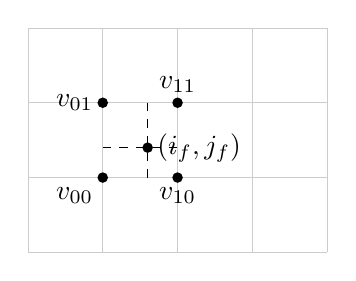
\begin{tikzpicture}[scale=0.95]
  \draw[step=1,gray!40,very thin] (0,0) grid (4,3);
  \fill (1,1) circle (2pt) node[below left] {$v_{00}$};
  \fill (2,1) circle (2pt) node[below] {$v_{10}$};
  \fill (1,2) circle (2pt) node[left] {$v_{01}$};
  \fill (2,2) circle (2pt) node[above] {$v_{11}$};
  \fill (1.6,1.4) circle (2pt) node[right] {$(i_f,j_f)$};
  \draw[dashed] (1.6,1) -- (1.6,2);
  \draw[dashed] (1,1.4) -- (2,1.4);
\end{tikzpicture}
\caption{Bilinear örneklemede kesirli indeksin dört komşu piksel merkeziyle ilişkilendirilmesi.
Boylam yönünde sarma, enlem yönünde kırpma uygulanır.}
\end{figure}

\subsection*{Büyüklük Dönüşümleri: DN \(\rightarrow\) Yükseklik/Yarıçap}
Ham IMG içeriği (etiket konvansiyonuna göre) ``DN'' olarak okunur ve bu ürün için tipik olarak km ölçeğindedir.
Modül, etiketten gelen \texttt{SCALING\_FACTOR} ve \texttt{OFFSET} ile:
\[
h_{\text{km}} = \text{DN}\cdot s,\qquad
r_{\text{km}} = h_{\text{km}} + r_0
\]
dönüşümünü uygular. Metre cinsinden çıktı için \(1000\) ile çarpılır.
\texttt{kind} parametresiyle (\texttt{height\_km}, \texttt{height\_m}, \texttt{radius\_km}, \texttt{radius\_m} vb.)
hangi büyüklüğün döndürüleceği seçilir.

\subsection*{Moon-fixed (x,y,z) Üzerinden Yükseklik Yardımcıları}
Dinamik tarafta sık ihtiyaç: Moon-fixed Kartezyen bir noktanın altındaki topografyayı bilmek
(örn. groundtrack/terrain clearance). Bu nedenle modül:
\begin{itemize}
  \item \texttt{latlon\_from\_xyz\_m}: Moon-fixed \((x,y,z)\rightarrow(\phi,\lambda,r)\),
  \item \texttt{height\_from\_xyz\_m}: bulunan \((\phi,\lambda)\) ile grid’den \texttt{height\_m} örnekleme
\end{itemize}
fonksiyonlarını sağlar. \texttt{method} ile nearest/bilinear seçimi yapılır.

\subsection*{Hızlandırma ve Doğrulama (Smoke-Test) Kancaları}
\texttt{numba} mevcutsa nearest/bilinear çekirdekleri JIT ile hızlandırılır; yoksa aynı mantık saf Python/Numpy ile çalışır
(doğruluk korunur, hız düşer).
Modülün CLI bölümünde ayrıca pratik doğrulamalar bulunur:
\begin{itemize}
  \item Etikete göre beklenen dosya boyutu ile gerçek IMG dosya boyutunun karşılaştırılması,
  \item Örnek bir (lat,lon) noktasında yükseklik/yarıçap çıktısı,
  \item Opsiyonel alt-örneklem istatistikleri (min/max gibi).
\end{itemize}

\begin{table}[H]
\centering
\caption{Topografya modülünün ana metodları.}
\begin{tabular}{p{0.34\linewidth} p{0.60\linewidth}}
\hline
\textbf{Metod} & \textbf{Çıktı / Not} \\
\hline
\texttt{parse\_ldem16\_label} & PDS3 etiketten gerekli alanları okur (\texttt{PDS3MapInfo}). \\
\texttt{TopographyGrid.open} & IMG’yi memmap veya tam yükleme ile açar. \\
\texttt{sample\_nearest} & (lat,lon) için nearest örnekleme; enlem kırpma + boylam sarma içerir. \\
\texttt{sample\_bilinear} & (lat,lon) için bilinear örnekleme; enlem kırpma + boylam sarma içerir. \\
\texttt{latlon\_from\_xyz\_m} & Moon-fixed \((x,y,z)\rightarrow(\phi,\lambda,r)\) dönüşümü. \\
\texttt{height\_from\_xyz\_m} & Moon-fixed \((x,y,z)\) altındaki topografik yüksekliği (m) döndürür. \\
\hline
\end{tabular}
\end{table}



% ====================== Perturbation Kernels =================
\newpage
\subsection{Pertürbasyon Çekirdekleri: \texttt{perturbation\_kernels.py}}
\label{subsec:perturbation_kernels}

\texttt{perturbation\_kernels.py} modülü, Ay-merkezli yörünge dinamiğinde \uline{merkezî Ay çekimi ve küresel harmoniklerin (SH) dışında kalan} bazı önemli pertürbasyon ivmelerini
hızlı, kararlı ve Numba-uyumlu biçimde hesaplayan çekirdek fonksiyonları içerir.

Bu modülün tasarım felsefesi bilinçli olarak
\textbf{``dumb + fast''} yaklaşımına dayanır:
\begin{itemize}
  \item Fonksiyonlar yalnızca konum/hız ve parametreleri alır,
  \item Doğrudan ivme $\mathbf{a}$ üretir,
  \item SPICE, ephemeris interpolasyonu, çerçeve dönüşümleri,
        karar/konfigürasyon mantığı bu katmanda \textbf{yer almaz}.
\end{itemize}
Hangi pertürbasyon terimlerinin etkinleştirileceği,
üst seviye dinamik katmanda (\texttt{dynamics\_kernel.py}) bayraklarla belirlenir.

\paragraph{Çerçeve varsayımı.}
Tüm vektörler aynı çerçevede verilmelidir
(önerilen: Ay-merkezli eylemsiz \texttt{J2000}):
\[
\mathbf{r}_{sc}\;(\text{Ay}\rightarrow\text{Araç}),\qquad
\mathbf{r}_{sun}\;(\text{Ay}\rightarrow\text{Güneş}),\qquad
\mathbf{r}_{earth}\;(\text{Ay}\rightarrow\text{Dünya}).
\]
Üretilen tüm ivmeler de aynı çerçevededir.
Bu varsayım modül içinde açıkça şart koşulur.

% ---------------------------------------------------------
\subsection*{Modellerin Özeti ve Yörüngeye Göre Önemi}

Tablo~\ref{tab:pert_models}, bu modülde yer alan pertürbasyon terimlerini,
ölçek davranışlarını ve hangi yörünge rejimlerinde daha baskın olduklarını özetler.

\begin{table}[H]
\centering
\caption{Pertürbasyon terimleri ve tipik önem dereceleri}
\label{tab:pert_models}
\small
\begin{tabular}{p{3.3cm} p{6.2cm} p{5.1cm}}
\hline
\textbf{Terim} & \textbf{Ölçek / davranış} & \textbf{Daha kritik olduğu rejimler} \\
\hline
3. cisim (Dünya/Güneş) &
$\sim \mu\, r / D^3$ (tidal/differential) &
HLO, NRHO, halo; uzun süreli propagasyon \\

SRP (cannonball) &
$\sim P_0(AU/d)^2 C_r(A/m)$; gölgede $0\!-\!1$ ölçek &
Yüksek $A/m$, CubeSat’ler, transfer yörüngeleri \\

Albedo (Lambert) &
$\sim P_{\odot@Moon}(R/r)^2\,\mathrm{phase}(\alpha)$ &
Düşük Ay yörüngeleri (LLO), güneş-altı taraf \\

Termal IR (basit) &
$\sim \varepsilon\sigma T^4/c \cdot (R/r)^2$ &
LLO; uzun süreli yarı-büyük eksen drift analizleri \\

GR 1PN &
$\mathcal{O}((v/c)^2)$ düzeyi &
Yüksek hassasiyetli OD / bilimsel çalışmalar \\
\hline
\end{tabular}
\end{table}

% ---------------------------------------------------------
\subsection*{Sayısal Koruyucular ve Yardımcı Fonksiyonlar}

Tüm çekirdek fonksiyonlar, \texttt{Numba} uyumlu küçük yardımcılar
(norm, dot, $1/r^3$ vb.) kullanır.
Özellikle:
\begin{itemize}
  \item $1/r^3$ türü ifadelerde $r$ çok küçükse,
        taşma veya NaN üretmemek için
        güvenli eşiklerle sıfır döndürülür.
  \item Fiziksel olmayan parametreler
        (negatif kütle, alan, $AU$, $P_0$ vb.)
        durumunda ilgili terim doğrudan sıfırlanır.
\end{itemize}
Bu korumalar, uzun süreli propagasyonda
``tek adımda çökme'' riskini ciddi biçimde azaltır.

% ---------------------------------------------------------
\subsection*{Ay Gölgesi: Konik Umbra/Penumbra Modeli}

SRP ve isteğe bağlı olarak albedo/termal terimlerinde,
Ay gölgesi \textbf{sonlu Güneş yarıçapını} içeren
konik umbra/penumbra modeliyle ele alınır.

Güneş yön birim vektörü:
\[
\hat{\mathbf{s}}=\frac{\mathbf{r}_{sun}}{\|\mathbf{r}_{sun}\|}.
\]
Uzay aracının gölge ekseni üzerindeki izdüşümü:
\[
\mathrm{proj}=\mathbf{r}_{sc}\cdot\hat{\mathbf{s}}.
\]
$\mathrm{proj}\ge 0$ ise araç güneş-altı taraftadır ve gölge yoktur ($s=1$).
Ay arkasında:
\[
x=-\mathrm{proj},\qquad
\rho=\left\|\mathbf{r}_{sc}-\mathrm{proj}\,\hat{\mathbf{s}}\right\|.
\]

Umbra ve penumbra yarıçapları benzer üçgenlerden türetilir:
\[
r_u(x)=R_{moon}\left(1-\frac{x}{L_u}\right),\qquad
r_p(x)=R_{moon}\left(1+\frac{x}{L_p}\right).
\]

Penumbra bölgesinde
\[
u=\frac{\rho-r_u}{r_p-r_u},\qquad
s(u)=3u^2-2u^3
\]
ile \textbf{yumuşak geçiş} sağlanır.
Bu, gölge sınırında ivmenin keskin sıçramasını önleyerek
integratör kararlılığını artırır.


% ---------------------------------------------------------
\subsection*{Model-1: Üçüncü Cisim Yerçekimi (Differential)}

\[
\mathbf{a}_{3B}=
\mu_B\left(
\frac{\mathbf{r}_B-\mathbf{r}_{sc}}{\|\mathbf{r}_B-\mathbf{r}_{sc}\|^3}
-
\frac{\mathbf{r}_B}{\|\mathbf{r}_B\|^3}
\right).
\]

Bu ifade, uzay aracının üçüncü cisme olan ivmesi ile
Ay merkezinin aynı cisme olan ivmesi arasındaki farkı alarak
\emph{tidal bileşeni} izole eder.

% ---------------------------------------------------------
\subsection*{Model-2: Güneş Işınım Basıncı (SRP)}

\[
\mathbf{a}_{SRP}
=
P_0\left(\frac{AU}{d}\right)^2
C_r\frac{A}{m}\hat{\mathbf{u}},
\qquad
\hat{\mathbf{u}}=\frac{\mathbf{r}_{sc}-\mathbf{r}_{sun}}{\|\mathbf{r}_{sc}-\mathbf{r}_{sun}\|}.
\]

SRP ivmesi, opsiyonel olarak gölge katsayısı $s$ ile ölçeklenir;
tam umbrada sıfırdır.

% ---------------------------------------------------------
\subsection*{Model-3: Ay Albedosu (Lambertian)}

Albedo ivmesi:
\[
\mathbf{a}_{alb}
=
P_{alb} C_r\frac{A}{m}\hat{\mathbf{r}},
\qquad
\hat{\mathbf{r}}=\frac{\mathbf{r}_{sc}}{\|\mathbf{r}_{sc}\|}.
\]

\[
P_{alb}
=
P_{\odot@Moon}\,
A_{moon}\left(\frac{R_{moon}}{r}\right)^2
\frac{1+\cos\alpha}{2}\,k_{L}.
\]

Varsayılan Lambert katsayısı $k_L=2/3$’tür;
test senaryolarında farklı değerler kullanılabilir.

% ---------------------------------------------------------
\subsection*{Model-4: Termal IR Yeniden-Işınımı}

Termal IR modeli, Ay yüzeyinin
gündüz/gece sıcaklıklarının
$T^4$ uzayında harmanlanmasıyla tanımlanır:
\[
T^4=
\mathrm{phase}_{day}T_{day}^4+
(1-\mathrm{phase}_{day})T_{night}^4.
\]

Eclipse sırasında yalnızca gündüz payı
gölge katsayısı $s$ ile ölçeklenir;
gece yayımı korunur.
Bu yaklaşım, ani enerji kopmalarını önler.

% ---------------------------------------------------------
\subsection*{Model-5: Genel Görelilik (1PN)}

\[
\mathbf{a}_{GR}=\frac{\mu}{c^2}\frac{1}{r^3}
\left[
\left(\frac{4\mu}{r}-v^2\right)\mathbf{r}
+4(\mathbf{r}\cdot\mathbf{v})\mathbf{v}
\right].
\]

Ay için çok küçük olmakla birlikte, uzun süreli hassas analizlerde
sistematik bir katkı sağlar.

% ---------------------------------------------------------
\subsection*{Toplama Yardımcısı ve Self-Test}

\texttt{accel\_perturbations(...)} fonksiyonu,
seçilen terimleri (3B, SRP, albedo, GR)
tek bir $\mathbf{a}_{pert}$ içinde toplar.

Dosya \texttt{\_\_main\_\_} altında
kapsamlı bir self-test bloğu içerir:
\begin{itemize}
  \item Gölge geometrisi ve SRP davranışı,
  \item Albedo ve termal faz ölçeklemesi,
  \item 3. cisim tidal limitleri,
  \item GR düzeltmesinin küçüklüğü,
  \item Ayrı ayrı hesaplanan ivmeler ile
        toplam fonksiyonun tutarlılığı.
\end{itemize}
Bu testler, modülün
uzun süreli propagasyonlar için
sayısal olarak güvenli olduğunu doğrular.



% ====================== Dinamik Çekirdek ======================
\newpage
\subsection{Dinamik Çekirdek: \texttt{dynamics\_kernel.py}}
\label{subsec:dynamics_kernel}

\texttt{dynamics\_kernel.py}, entegratörün doğrudan çağırdığı \textbf{durum türevi (RHS)} ve \textbf{ivme} fonksiyonlarını üretir. Temel hedef; farklı fizik modellerini (\texttt{gravity\_kernels.py}, ve  newline\texttt{perturbation\_kernels.py}) tek bir tutarlı arayüz altında birleştirirken, \textbf{}{zaman/çerçeve tutarlılığını} zorunlu kılmaktır. Dışarıya üç ana yapı sunar:

\begin{itemize}
  \item \texttt{DynamicsContext}: sabitler, SH katsayıları, ephemeris tabloları ve bayraklar için bağlam (context).
  \item \texttt{make\_rhs(ctx)}: genel amaçlı ODE çözücüleri için \(\dot{\mathbf{y}}=f(t,\mathbf{y})\) üretir.
  \item \texttt{make\_accel(ctx)}: sabit adımlı/simetrik integratörler için yalnız \(\mathbf{a}(t,\mathbf{y})\) döndürür.
\end{itemize}

\subsection*{Durum Tanımı ve Referans Çerçeveler}
Bu modülde durum vektörü Ay-merkezli \textbf{eylemsiz} çerçevede tanımlıdır:
\begin{equation}
\mathbf{y}=
\begin{bmatrix}
\mathbf{r}_I\\
\mathbf{v}_I
\end{bmatrix}
=
\begin{bmatrix}
x_I & y_I & z_I & v_{xI} & v_{yI} & v_{zI}
\end{bmatrix}^{T},
\qquad
[\mathbf{r}_I]=\mathrm{m},\ \ [\mathbf{v}_I]=\mathrm{m\,s^{-1}}.
\end{equation}
Hareket denklemi:
\begin{equation}
\dot{\mathbf{r}}_I=\mathbf{v}_I,
\qquad
\dot{\mathbf{v}}_I=\mathbf{a}_{\mathrm{total}}(t,\mathbf{r}_I,\mathbf{v}_I).
\label{eq:dyn_ode}
\end{equation}

\paragraph{Neden inertial + fixed birlikte?}
Sferik harmonik (SH) yerçekimi katsayıları \textbf{Ay-sabit (body-fixed)} çerçevede tanımlıdır.
Bu yüzden SH ivmesi \(\mathbf{a}_{SH}\) hesaplanırken konum \(\mathcal{I}\rightarrow\mathcal{F}\) döndürülür,
ivme fixed’de üretilir ve tekrar \(\mathcal{F}\rightarrow\mathcal{I}\) döndürülerek entegrasyona eklenir.
Bu adımı atlamak, fiziksel olmayan periyodik hatalara ve uzun dönemde ciddi drift’e yol açabilir.

\subsection*{Zaman Eşlemesi: Entegratör Zamanı \texorpdfstring{\(\rightarrow\)}{->} Tablo Zamanı}
Ephemeris tabloları \(\Delta t_{\mathrm{ephem}}\) ile örneklenmiştir.
Kod, integratörden gelen zamanı tek bir referansla hizalamak için
\begin{equation}
t_{\mathrm{rel}} = t - t_0
\end{equation}
ofsetini uygular (burada \(t_0\) bağlamda \texttt{ctx.t0\_s} olarak taşınır).
Böylece ``entegratör zamanı'' ile ``tablo zamanı'' karışmaz; özellikle farklı başlangıç senaryolarında
aynı ephemeris tablosunu güvenle kullanmak mümkün olur.

\subsection*{Çerçeve Dönüşümü: Quaternion + SLERP}
SH hesabı için inertial\(\rightarrow\)fixed dönüşümü, zamanla değişen birim quaternion tablosu ile yapılır.
Tablo ara değerlemesi \emph{SLERP} ile gerçekleştirilir; böylece dönüşler kesintisiz ve düzgün olur:
\begin{equation}
\mathbf{r}_F = \mathcal{R}\big(q_{I\rightarrow F}(t_{\mathrm{rel}})\big)\,\mathbf{r}_I,
\qquad
\mathbf{a}_I = \mathcal{R}\big(q_{I\rightarrow F}(t_{\mathrm{rel}})\big)^{T}\,\mathbf{a}_F.
\end{equation}
SLERP seçimi, özellikle yüksek açısal hızlarda lineer quaternion enterpolasyonunun üretebileceği
norm kayması ve ``yön sıçraması'' problemlerini azaltır.

\subsection*{Toplam İvme: Modüler Toplam ve Bayraklar}
Toplam ivme, açık/kapalı seçilebilen terimlerin toplamı olarak ele alınır:
\begin{equation}
\mathbf{a}_\text{total}=
\underbrace{\mathbf{a}_{2b}+\mathbf{a}_\text{SH}}_{\text{Ay yerçekimi}}
+\underbrace{\mathbf{a}_{3b,E}+\mathbf{a}_{3b,S}}_{\text{3. cisim (Dünya+Güneş)}}
+\underbrace{\mathbf{a}_\text{SRP}+\mathbf{a}_\text{alb}+\mathbf{a}_\text{th}}_{\text{radyasyon tabanlı}}
+\underbrace{\mathbf{a}_\text{tide}+\mathbf{a}_{J2,E}}_{\text{opsiyonel ince düzeltmeler}}
+\underbrace{\mathbf{a}_\text{GR}}_{\text{1PN (ops.)}}.
\label{eq:atotal_sum}
\end{equation}

Hangi terimlerin ekleneceği \texttt{ctx.flags} ile belirlenir (ör.\ \texttt{SH\_GRAVITY},
\texttt{THIRD\_BODY}, \texttt{SRP}, \texttt{ALBEDO}, \texttt{THERMAL\_IR}, \texttt{SOLID\_TIDES},
\texttt{EARTH\_J2}, \texttt{GR\_1PN}, \texttt{USE\_SPICE}). Bayraklar arası bağımlılıklar
\textbf{koşum başlamadan} kontrol edilerek mantıksız kombinasyonlarda açık hata verilir.

\begin{table}[H]
\centering
\caption{Bayraklar, bağımlılıklar ve pratik önem.}
\begin{tabular}{p{3.2cm} p{5.0cm} p{6.6cm}}
\hline
\textbf{Terim / Bayrak} & \textbf{Gereksinim} & \textbf{Ne zaman daha önemli?} \\
\hline
\texttt{SH\_GRAVITY} &
\texttt{USE\_SPICE=True} ve \(q_{I\rightarrow F}(t)\) tablosu &
\textbf{LLO/çok alçak irtifa:} mascon etkileri, periselene kayması, uzun dönem hata birikimi.\\
\texttt{THIRD\_BODY} &
\(\mathbf r_E(t), \mathbf r_S(t)\) tabloları + \(\mu_E,\mu_S\) &
\textbf{HLO/NRHO/halo rejimleri:} Ay merkezi ivme zayıflarken 3. cisim tidal etkileri göreli büyür.\\
\texttt{SRP}/\texttt{ALBEDO}/\texttt{THERMAL\_IR} &
Güneş vektörü tablosu \textbf{ve pratikte} \texttt{THIRD\_BODY} altyapısı &
\textbf{Yüksek \(A/m\)} ve uzun süreli propagasyon; gölge geçişlerinde enerji/eleman drift’i.\\
\texttt{SOLID\_TIDES} &
\texttt{THIRD\_BODY} + Love \(k_2\) &
Uzun dönem hassas analiz; küçük ama sistematik etkiler.\\
\texttt{EARTH\_J2} &
\texttt{THIRD\_BODY} + Dünya eksen/J2 parametreleri &
Yüksek doğruluk isteyen senaryolar; genelde ikincil bir düzeltme.\\
\texttt{GR\_1PN} &
\(c\) ve \(\mu_M\) &
Çok hassas uzun dönem analiz; küçük ama yönlü/sistematik katkı.\\
\hline
\end{tabular}
\end{table}

\subsection*{Ay Yerçekimi: 2-Body + SH}
SH kapalıysa yalnız merkezi çekim kullanılır:
\begin{equation}
\mathbf{a}_{2b} = -\mu_M\frac{\mathbf{r}_I}{\|\mathbf{r}_I\|^3}.
\end{equation}
SH açıksa iş akışı şu şekildedir:
\begin{enumerate}
  \item \(\mathbf{r}_I \xrightarrow{q(t)} \mathbf{r}_F\) (inertial\(\rightarrow\)fixed).
  \item \(\mathbf{a}_F \leftarrow \texttt{sh\_accel\_fixed\_numba}(\mathbf{r}_F)\).
  \item \(\mathbf{a}_F \xrightarrow{q(t)^\ast} \mathbf{a}_I\) (fixed\(\rightarrow\)inertial) ve toplam ivmeye eklenir.
\end{enumerate}
Bu tasarım, SH’nin tanımlı olduğu çerçeveyi zorunlu kılar ve çerçeve hatalarını daha en baştan engeller.

\subsection*{Üçüncü Cisim (Dünya+Güneş): Diferansiyel Noktasal Model + Catmull--Rom}
Üçüncü cisim ivmesi Ay-merkezli diferansiyel formda yazılır:
\begin{equation}
\mathbf{a}_{3b}(\mathbf{r})=
\mu_b\left(
\frac{\mathbf{r}_b-\mathbf{r}}{\|\mathbf{r}_b-\mathbf{r}\|^3}
-
\frac{\mathbf{r}_b}{\|\mathbf{r}_b\|^3}
\right),
\label{eq:third_body}
\end{equation}
burada \(\mathbf{r}\) uzay aracının Ay-merkezli konumu, \(\mathbf{r}_b\) ise Ay\(\rightarrow\)cisim (Dünya/Güneş) vektörüdür.
\(\mathbf r_E(t)\) ve \(\mathbf r_S(t)\) tabloları üzerinde ara değerleme yapılırken
\textbf{Catmull--Rom} benzeri sürekli-türevli bir şema tercih edilir.
Bu seçim, özellikle uzun süreli koşularda ivme girişlerindeki keskin kırılmaları azaltarak integratör kararlılığını iyileştirir.

\subsection*{SRP, Albedo, Termal IR: Modüler Çağrılar ve Gölge}
Radyasyon tabanlı terimler Güneş doğrultusuna bağlıdır ve bu nedenle Güneş vektörü tablosu gerektirir.
Bu modül, ilgili ivmeleri \texttt{perturbation\_kernels.py} içindeki çekirdek fonksiyonlar üzerinden çağırır:
\begin{itemize}
  \item \textbf{SRP:} cannonball yaklaşımı; gölgede etkinlik \(s\in[0,1]\) ile ölçeklenir.
  \item \textbf{Albedo:} basit Lambert varsayımı + faz fonksiyonu.
  \item \textbf{Termal IR:} gündüz/gece harmanlı yüzey yayımı modeli.
\end{itemize}
\paragraph{Gölge hesabı.}
\texttt{ECLIPSE} bayrağı bağlamda bulunsa da, uygulamada SRP/Albedo/Termal açıkken gölge katsayısının
hesabı devrededir; böylece umbra/penumbra geçişlerinde ani sıçrama yerine yumuşak bir ölçekleme uygulanır.

\subsection*{Opsiyonel İnce Düzeltmeler: Earth J2 ve Solid Tides}
İhtiyaç halinde iki ek düzeltme açılabilir:
\begin{itemize}
  \item \textbf{Earth J2 diferansiyel düzeltmesi:} Dünya alanının J2 katkısı Ay-merkezli diferansiyel düzeltme olarak eklenir.
  \item \textbf{Solid-body tides:} Love sayısı \(k_2\) ile parametrik, Dünya (ve opsiyonel Güneş) tarafından uyarılan gelgit ivmeleri eklenir.
\end{itemize}
Bu terimler genellikle SH’ye göre küçük kalsa da, uzun dönem hassas analizlerde sistematik drift oluşturabilir.

\subsection*{Genel Görelilik: 1PN Schwarzschild (Ops.)}
Opsiyonel 1PN terimi Ay’ın merkezi alanına hız-bağımlı bir düzeltme ekler:
\begin{equation}
\mathbf{a}_\text{GR} = \frac{\mu_M}{c^2\,r^3}
\left[
\left(\frac{4\mu_M}{r}-v^2\right)\mathbf{r} + 4(\mathbf{r}\cdot\mathbf{v})\mathbf{v}
\right].
\end{equation}
Hız bağımlılığı nedeniyle, sıkı ``tam simplektik'' varsayımlar zayıflayabilir; bu yüzden yalnız ihtiyaç olduğunda açılması önerilir.

\subsection*{Güvenlik Kontrolleri ve Tipik Hata Kaynakları}
Koşum başlamadan önce şu mantıksal kontroller yapılır:
\begin{itemize}
  \item \textbf{SH için dönüşüm şartı:} \texttt{SH\_GRAVITY=True} iken \texttt{USE\_SPICE=True} ve yeterli uzunlukta \(q_{I\rightarrow F}\) tablosu gerekir.
  \item \textbf{3. cisim altyapısı:} \texttt{THIRD\_BODY=True} iken Earth/Sun tabloları ve \(\mu_E,\mu_S\) pozitif olmalıdır.
  \item \textbf{SRP/Albedo/Termal bağımlılığı:} Bu terimler açıkken Güneş vektörü tablosu zorunludur; pratikte bu da \texttt{THIRD\_BODY} altyapısını gerektirir.
  \item \textbf{Tides ve Earth J2:} Bu düzeltmeler için de Earth/Sun tabloları gerektiğinden \texttt{THIRD\_BODY} kapalıyken açılmaz.
\end{itemize}

\paragraph{Kuvvet ayrıştırma (\texttt{make\_accel\_breakdown}).}
Analiz/raporlama için toplam ivmeyi bileşenlerine ayıran bir yardımcı da sağlanır:
\(\{\texttt{"SH"},\texttt{"Earth"},\texttt{"Sun"},\texttt{"SRP"},\ldots,\texttt{"Total"}\}\).
Bu çıktı, hangi perturbasyonun hangi zamanda baskın olduğunu görselleştirmeyi kolaylaştırır.

\begin{figure}[H]
\centering
\fbox{
\begin{minipage}{0.95\linewidth}
\textbf{RHS değerlendirme akışı (tek adım)}\\[2pt]
1) \(t_{\mathrm{rel}}=t-t_0\) \\ 
2) (ops.) \(q(t_{\mathrm{rel}})\) ile \(\mathbf{r}_I\rightarrow\mathbf{r}_F\) \\ 
3) (ops.) \(\mathbf{a}_F\leftarrow \text{SH}(\mathbf{r}_F)\), sonra \(\mathbf{a}_F\rightarrow\mathbf{a}_I\) \\ 
4) (ops.) \(\mathbf{r}_E(t),\mathbf{r}_S(t)\) ara değerle (Catmull--Rom) ve \(\mathbf{a}_{3b}\) ekle \\ 
5) (ops.) SRP/Albedo/Termal + gölge katsayısı \(s\in[0,1]\) \\ 
6) (ops.) Earth J2 / solid tides / GR düzeltmeleri \\ 
7) \(\dot{\mathbf{y}}=[\mathbf{v}_I;\mathbf{a}_\text{total}]\)
\end{minipage}
}
\caption{\texttt{dynamics\_kernel.py} içinde RHS değerlendirmesinin modüler akışı.}
\end{figure}

\subsection*{Dosya İçi Self-Test}
Dosya doğrudan çalıştırıldığında (opsiyonel) basit bir 2-body tutarlılık testi sunar:
SH ve 3. cisim kapalıyken, üretilen ivmenin \(-\mu\mathbf{r}/r^3\) ile uyumlu olduğu
hem \texttt{make\_rhs} hem \texttt{make\_accel} üzerinden doğrulanır.


% ====================== Propagator ======================
\newpage
\subsection{Yörünge Yayılımı: \texttt{propagator.py}}
\label{subsec:propagator}

\subsubsection*{Amaç ve Kapsam}
\texttt{propagator.py}, \texttt{dynamics\_kernel.make\_rhs(ctx)} tarafından üretilen
\(\dot{\mathbf y}=\mathbf f(t,\mathbf y)\) sağ tarafını seçilen nümerik yöntemle entegre ederek
durum vektörü tarihçesini \(\mathbf y(t)=[\mathbf r,\mathbf v]\) üretir.
Buna ek olarak modül:
(i) Nyquist tabanlı adım üst sınırıyla yüksek dereceli SH alanlarında örnekleme güvenliği,
(ii) impact/periselene/aposelene ve topografya-duyarlı hybrid impact event’leri,
(iii) seyrek ``heartbeat'' loglama,
(iv) isteğe bağlı 2-cisim baseline çözümü,
(v) uzun koşular için chunk’lı entegrasyon + checkpoint ve ``graceful stop''
mekanizmalarını sağlar.

Bu tasarım, hem doğruluk teşhisini hem de uzun süreli simülasyonlarda operasyonel sağlamlığı artırır.
Modül içe aktarımlarını, proje ``package'' olarak çalıştırıldığında ve tek dosya (script) olarak çalıştırıldığında
uyumlu olacak şekilde düzenler.

\subsubsection*{Konfigürasyon: \texttt{PropagatorConfig}}
Propagator davranışı tek bir yapılandırma sınıfı ile taşınır. Temel alanlar Tablo~\ref{tab:prop_cfg}’de özetlenmiştir.

\begin{table}[H]
\centering
\caption{\texttt{PropagatorConfig} alanları ve kullanım amacı}
\label{tab:prop_cfg}
\begin{tabular}{p{0.28\linewidth} p{0.18\linewidth} p{0.45\linewidth}}
\hline
\textbf{Alan} & \textbf{Tipik} & \textbf{Amaç} \\
\hline
\texttt{sim\_hours}, \texttt{sim\_days}, \texttt{t0\_s} & 72 h & Simülasyon süresi ve başlangıç zamanı; \texttt{sim\_days} verilirse \texttt{sim\_hours}’u override eder. \\
\texttt{output\_dt\_s}, \texttt{max\_points\_cap} & 60 s & Kayıt/plot ızgarası yoğunluğu ve bellek yumuşak sınırı. \\
\texttt{method}, \texttt{rtol}, \texttt{atol} & DOP853 & Adaptif \texttt{solve\_ivp} yöntemi ve toleranslar. \\
\texttt{user\_max\_step\_s} & None & Kullanıcı üst adım sınırı; Nyquist ile birlikte \(\min(\cdot)\) alınır. \\
\texttt{nyquist\_safety\_div}, \texttt{nyquist\_v\_margin} & 4.0, 1.10 & Nyquist adım hesabında güvenlik payları. \\
\texttt{impact\_alt\_km}, \texttt{enable\_peri\_apo\_events} & 5 km & Çarpma eşiği ve peri/apo event’lerini aç/kapat. \\
\texttt{heartbeat\_hours}, \texttt{verbose} & 6 h & Seyrek loglama/izleme. \\
\texttt{compute\_2body\_baseline} + baseline toleransları & True & 2-cisim referans çözüm ile kıyas (enerji drift teşhisi). \\
\texttt{stop\_file} & None & Dosya varlığıyla ``cooperative stop'' tetikleme (graceful stop). \\
\texttt{checkpoint\_path}, \texttt{checkpoint\_every\_chunk} & None & Süreç sırasında kısmi yörüngeyi \texttt{.npz} olarak atomik yazma. \\
\texttt{solve\_ivp\_chunk\_s} & None & Adaptif çözücüde zaman aralığını parçalara bölerek ilerleme (uzun koşu sağlamlığı). \\
\hline
\end{tabular}
\end{table}

\subsubsection*{Adım Boyu Seçimi: Nyquist + Kullanıcı Üst Sınırı}
Yüksek derece sferik harmonik (SH) alanları, uzaysal olarak daha kısa dalga boyları içerir.
Araç düşük irtifada hızlı hareket ederken, entegratör adımı fazla büyük seçilirse
bu uzaysal detay zamansal örneklemede aliasing üretebilir.
Bu nedenle propagator, \texttt{math\_utils.nyquist\_max\_step\_s} fonksiyonuyla güvenli bir üst sınır önerir:
\[
\lambda_N \approx \frac{2\pi R}{N},\qquad
T_\lambda \approx \frac{\lambda_N}{v_{\max}},\qquad
\Delta t_{\max} \lesssim \frac{T_\lambda}{\text{safety\_div}}.
\]
Hız için muhafazakâr bir üst sınır:
\[
v_{\max} \approx \sqrt{\frac{\mu}{r_{\min}}}\,\text{v\_margin}
\]
şeklinde alınır.

Propagator içinde seçilen adım üst sınırı:
\[
\Delta t_{\max}=\begin{cases}
\Delta t_{\text{Nyq}} & \text{eğer } \texttt{user\_max\_step\_s}=\varnothing,\\
\min(\texttt{user\_max\_step\_s},\,\Delta t_{\text{Nyq}}) & \text{aksi halde}
\end{cases}
\]
olarak uygulanır ve \texttt{verbose} açıksa ekrana raporlanır.

\paragraph{Ephemeris ve çıktı örnekleme tutarlılığı.}
Kod, ephemeris tablosu örnekleme aralığının (\texttt{ctx.dt\_ephem\_s})
seçilen \(\Delta t_{\max}\)’tan daha kaba olması durumunda uyarı basar;
benzer şekilde \texttt{output\_dt\_s} çok büyükse plot/kayıt çözünürlüğünün kaba olacağı belirtilir.

\subsubsection*{Entegrasyon Modları: Adaptif (\texttt{solve\_ivp}) ve Sabit Adım (Semplektik)}
Varsayılan yaklaşım, \texttt{scipy.integrate.solve\_ivp} tabanlı adaptif entegrasyondur.
Bu mod, tolerans kontrolüyle adım boyunu otomatik ayarlayarak geniş senaryo yelpazesinde güvenilir sonuç üretir.

Buna ek olarak modül, sabit adım gereken koşular için
Velocity--Verlet (KDK) ve 4.\ mertebe Yoshida bileşimi gibi şemaları içerir:
\begin{itemize}
\item \textbf{VV (Velocity--Verlet):} otonom ve korunumlu \( \mathbf a=\mathbf a(\mathbf r) \) modellerinde enerji davranışı açısından avantajlıdır.
\item \textbf{Y4 (Yoshida-4):} VV adımının 4.\ mertebe kompozisyonudur (VV\((w_1 h)\)\(\rightarrow\)VV\((w_0 h)\)\(\rightarrow\)VV\((w_1 h)\)). 
\end{itemize}
Hız-bağımlı terimler açıldığında ``tam semplektiklik'' zayıflasa da şemalar pratikte kararlı biçimde çalışır.

\subsubsection*{Event Sistemi: Impact, Periselene, Aposelene ve Hybrid Impact}
Propagator, \texttt{events.py} içindeki event üreticilerini kullanır:
\begin{itemize}
  \item \textbf{Impact (terminal):} \(\|\mathbf r\|-R_\text{ref} - h_{\text{impact}}=0\) eşitliğini aşağı yönde kestiğinde durur.
  \item \textbf{Periselene/Aposelene (non-terminal):} \(\mathbf r\cdot\mathbf v\) işaret değişiminden radyal hızın sıfırlandığı noktalar yakalanır.
  \item \textbf{Hybrid impact (terminal):} Yüksek irtifada küresel referans yarıçapı ile hızlı kontrol;
        belirli bir \texttt{switch\_alt} altına inince DEM/topografya üzerinden gerçek yüzey açıklığı (terrain clearance) ile durdurma.
\end{itemize}
Hybrid yaklaşım, çok alçak irtifalarda topografyayı ihmal etmenin ürettiği ``erken/geç çarpışma'' hatasını azaltmak için tasarlanmıştır.

\subsubsection*{Heartbeat İzleme}
Uzun koşularda her adımın loglanması pahalıdır.
Heartbeat mekanizması, \texttt{heartbeat\_hours} aralığında kısa bir özet basarak
entegrasyonun ilerlemesini ve irtifa trendlerini izlemeyi sağlar.

\subsubsection*{Uzun Koşular için Sağlamlık: Chunk’lama, Checkpoint ve Graceful Stop}
Çok uzun simülasyonlarda tek seferde \texttt{solve\_ivp} çağrısı yapmak yerine,
zaman aralığını parçalara bölerek ``chunk'' bazlı ilerlemek daha sağlam bir stratejidir.
Bu modül:
\begin{itemize}
  \item \texttt{solve\_ivp\_chunk\_s} ile adaptif entegrasyonu parçalara böler,
  \item her chunk sonunda istenirse \texttt{checkpoint\_path} altına kısmi sonuçları \texttt{.npz} olarak yazar,
  \item \texttt{stop\_file} mevcutsa bir sonraki güvenli noktada simülasyonu temiz şekilde sonlandırır.
\end{itemize}
Checkpoint yazımı atomik biçimde yapılarak (geçici dosya + replace),
yarım dosya veya bozuk checkpoint riski azaltılır.

\subsubsection*{Opsiyonel 2-Cisim Baseline (Kıyas)}
İsteğe bağlı olarak sadece merkezi çekimle:
\[
\ddot{\mathbf r}=-\mu\frac{\mathbf r}{\|\mathbf r\|^3}
\]
2-cisim baseline çözümü üretilir.
Bu çözüm, enerji drift’i / tolerans ayarı / model karmaşıklığı ayrımı için pratik bir referanstır.

\subsection*{Core Katmanı ile Uyum}
\texttt{propagator.py}, çekirdek dinamik katmandan yalnızca
\(\mathbf f(t,\mathbf y)\) arayüzünü (\texttt{make\_rhs}) tüketir;
yerçekimi ve pertürbasyon detayları \texttt{dynamics\_kernel.py} içinde soyutlanmıştır.
Event seti \texttt{events.py} tarafından üretildiği için propagator,
``durma/kritik nokta tespiti'' mantığını fizik modelinden ayrı tutar.
Bu sayede yeni pertürbasyonlar eklendiğinde propagator tarafında değişiklik ihtiyacı minimum olur.



% ============================================================
% ======================== UTILS ==============================
% ============================================================
\newpage
\section{UTILS Klasörü: Sayısal Yardımcılar, Olay Yakalama ve Raporlama}
\label{sec:utils_folder}

\texttt{UTILS} klasörü, çekirdek (\texttt{core/}) katmanda üretilen dinamik/ivme çıktılarının
simülasyon boyunca güvenli biçimde kullanılmasını, olayların (event) yakalanmasını ve sonuçların görselleştirilip raporlanmasını sağlayan yardımcı modülleri içerir. Bu katman, fiziksel modeli yeniden tanımlamaz; onun yerine dönüşüm, kontrol, kayıt, analiz ve sunum işlevlerini üstlenerek simülasyon hattını uçtan uca tamamlar.

Klasör içerisinde yer alan temel bileşenler şunlardır:

\begin{itemize}
    \item \textbf{math\_utils.py}: Sayısal dönüşümlerin ve geometrik yardımcıların toplandığı modüldür.
    Kuaterniyon işlemleri (normalize, çarpım, ters/konjüge), dönüşüm matrisleri, eylemsiz/sabit çerçeve dönüşümleri ve sık kullanılan yörünge eleman dönüşümleri (ör. durum vektörü $\leftrightarrow$ Kepler elemanları gibi) bu katmanda standartlaştırılır. Amaç, koordinat/temsil tutarlılığını tek bir kaynaktan yönetmektir.

    \item \textbf{events.py}: Entegrasyon sırasında fiziksel olarak anlamlı sınır durumlarını yakalamak için
    olay fonksiyonlarını içerir. Periapsis/periselene tespiti, çarpışma (yüzey kesişimi), irtifa eşiği geçişi veya belirli bir geometrik koşulun sağlanması gibi kriterler,
    integratörün event arayüzüne uygun şekilde tanımlanır.
    Böylece ``simülasyon bitti mi?'' veya ``kritik bir eşik aşıldı mı?'' soruları sistematik biçimde yönetilir.

    \item \textbf{postprocess.py}: Ham zaman serilerini mühendislik açısından anlamlı çıktılara çeviren
    post-process katmanıdır. Yörünge elemanlarının zamana göre çıkarılması, enerji/açısal momentum gibi korunum metrikleri, sapma/istatistik özetleri, filtreleme/yeniden örnekleme ve çıktı formatlama bu modülde toplanır. Bu ayrım, çekirdek simülasyon kodunu ``temiz'' tutar ve analiz kısmını izole eder.

    \item \textbf{styling.py}: Görsel çıktıların ortak stil ayarlarını standardize eder. Renk paleti, yazı tipi boyutları, çizgi/ızgara ayarları, figür boyutları gibi parametreler tek yerde tanımlanarak tüm grafiklerin aynı görsel dilde üretilmesi sağlanır. Rapor kalitesi ve tutarlılık açısından pratikte çok faydalıdır.

    \item \textbf{plotting.py}: Simülasyon çıktılarının grafiklere dönüştürüldüğü katmandır. Zaman serileri (ör. $r(t)$, $v(t)$, elemanlar), korunum hataları, üçüncü-cisim mesafeleri, aydınlanma/gölge durumları gibi çıktılar
    modüler fonksiyonlarla üretilir; \texttt{styling.py} ile uyumlu çalışacak şekilde tasarlanır.

    \item \textbf{report\_manager.py}: Sonuçların raporlanmasını yöneten üst seviye modüldür.
    Grafiklerin, özet tabloların ve seçilmiş metriklerin bir rapor çıktısında birleştirilmesi,
    çıktı klasörü organizasyonu, otomatik isimlendirme/sürümleme ve
    ``tek komutla çalıştır $\rightarrow$ çıktı üret'' akışının tamamlanması burada ele alınır.

    \item \textbf{threeD\_animation.py}: 3B yörünge animasyonu ve görselleştirme katmanıdır.
    Yörünge izinin 3B uzayda çizdirilmesi, isteğe bağlı olarak Ay yüzeyi/topografya ile birlikte
    kamera takibi, hızlandırılmış oynatma ve çıktı video/gif üretimi gibi işlevleri kapsar.
    Bu modül, özellikle sunum ve sezgisel doğrulama (ör. çarpışma geometrisi) açısından değerlidir.
\end{itemize}

\subsection*{Teknik Altyapı Notları}
\texttt{UTILS} katmanı, performansı kritik çekirdek döngülerden ziyade
\textbf{doğruluk, tutarlılık ve tekrar kullanılabilirlik} hedefiyle tasarlanmıştır.
Bununla birlikte:
\begin{itemize}
    \item Sık çağrılan düşük seviyeli hesaplar (ör. kuaterniyon normlama, temel dönüşümler, basit metrikler)
    uygun olduğunda \texttt{Numba} ile hızlandırılabilir; ancak bu katmanda öncelik
    okunabilirlik + güvenli arayüz dengesidir.
    \item Olay (event) fonksiyonları, integratörün kök-bulma mantığıyla uyumlu olacak şekilde
    sürekli (mümkün olduğunca pürüzsüz) tanımlanır; böylece yanlış tetikleme veya kararsız event davranışı azaltılır.
    \item Post-process ve görselleştirme adımları, çekirdek simülasyonu etkilemeyecek biçimde
    ayrık tutulur; bu sayede aynı ham veriden farklı rapor/plot setleri üretmek kolaylaşır.
    \item Çıktı üretim hattında (grafik/rapor/animasyon) ortak stil ve dosya organizasyonu
    standartlaştırılarak, deneylerin karşılaştırılabilirliği ve tekrar üretilebilirliği güçlendirilir.
\end{itemize}


% ================== Olay (Event) Yardımcıları ==================
\newpage
\subsection{Olay (Event) Yardımcıları: \texttt{events.py}}
\label{subsec:events}

Bu modül, yörünge entegrasyonu sırasında \textbf{fiziksel veya operasyonel koşulların} zaman içinde \textbf{tespit edilmesini} sağlayan \textbf{event üreticilerini} içerir. Amaç, \texttt{solve\_ivp} gibi genel amaçlı ODE çözücülerine,
simülasyon bağlamından kopmadan fakat yalın bir arayüzle
olay (event) tanımları sunmaktır.

Tasarım prensibi şudur:
\begin{quote}
“Entegratör yalnızca \(g(t,\mathbf{y})\) ister; gerekli geometri ve bağlam closure üzerinden enjekte edilir.”
\end{quote}

Bu sayede event fonksiyonları:
\begin{itemize}
  \item entegratör API’sini bozmadan çalışır,
  \item SPICE, ephemeris veya topo gibi ağır bağımlılıkları doğrudan içermez,
  \item test edilebilir ve yeniden kullanılabilir kalır.
\end{itemize}

Tüm event’ler SciPy standardına uygun olarak
\[
g(t,\mathbf{y}) \rightarrow \mathbb{R}
\]
biçimindedir ve opsiyonel olarak
\texttt{terminal} ve \texttt{direction} özniteliklerini taşır.

% ---------------------------------------------------------
\subsection*{Temel Event Türleri (Kararlı ve Sık Kullanılan)}

Bu gruptaki event’ler, klasik yörünge analizi için en sık kullanılan ve
sayısal olarak en kararlı tanımlardır.

\begin{itemize}
  \item \textbf{Impact / Altitude Event} \\
  Referans yarıçapına göre irtifa eşik geçişi:
  \[
  g(t,\mathbf{y}) = \|\mathbf{r}\| - R_{\text{ref}} - h_{\text{impact}}
  \]
  Aşağı yönlü geçişte tetiklenir (\texttt{direction = -1}).

  \item \textbf{Hybrid Impact Event} \\
  Yüksek irtifada küresel referans yarıçapı,
  alçak irtifada ise \texttt{topo\_manager} üzerinden \textbf{gerçek yerel yüzey}
  kullanılır. Bu yaklaşım:
  \begin{itemize}
    \item DEM sorgularını sadece gerektiğinde yapar,
    \item alçak irtifada topo kaynaklı erken/geç çarpışma hatalarını azaltır.
  \end{itemize}

  \item \textbf{Periselene / Aposelene} \\
  Klasik \( \mathbf{r}\cdot\mathbf{v}=0 \) koşuluna dayanır:
  \begin{itemize}
    \item periselene: negatiften pozitife geçiş,
    \item aposelene: pozitiften negatife geçiş.
  \end{itemize}
  Başlangıç anındaki sahte kökleri önlemek için küçük bir zaman koruması
  (\texttt{t\_guard}) uygulanır.

  \item \textbf{Yarıçap ve SOI Event’leri} \\
  Genel amaçlı yarıçap geçişleri ve basit bir
  \emph{sphere-of-influence} sınırı (geometrik tanım).
\end{itemize}

% ---------------------------------------------------------
\subsection*{Gelişmiş Geometrik ve Operasyonel Event’ler}

Bu event’ler, görev analizi ve operasyonel kısıtlar için tasarlanmıştır.Çoğu, zamanla değişen geometriyi closure yoluyla alır.

\paragraph{Terminatör Geçişi (Gündüz/Gece Sınırı).}
Uzay aracının alt-noktasının Ay üzerinde gündüz/gece sınırını geçmesi:
\[
g(t)=\hat{\mathbf{r}}_{\text{bf}}\cdot\hat{\mathbf{s}}_{\text{bf}}=0
\]
Burada hem konum hem Güneş yönü Moon-fixed çerçeveye dönüştürülür.
Bu event, güç/termal analizlerde kritik rol oynar.

\paragraph{Güneş Tutulması (Solar Eclipse).}
Uzay aracı ile Güneş arasındaki görüş hattının Ay ve/veya Dünya tarafından engellenmesi, doğru parça–küre kesişimi geometrisiyle test edilir.
Bu tanım:
\begin{itemize}
  \item Güneş’i noktasal kabul eder (hard shadow),
  \item Ay ve Dünya engellemelerini ayrı ayrı hesaba katabilir.
\end{itemize}

\paragraph{Maksimum Tutulma Süresi.}
Ardışık tutulma süresi izlenir ve belirli bir eşik aşılırsa event tetiklenir. Bu, batarya/termal güvenlik için bir operasyonel koruma mekanizmasıdır. Event, closure içinde küçük bir durum (state) tutarak süreyi entegre eder.

\paragraph{Düğüm (Node) Geçişleri.}
Referans bir düzleme göre:
\begin{itemize}
  \item çıkan düğüm,
  \item inen düğüm,
  \item veya her ikisi
\end{itemize}
tespit edilebilir. Varsayılan referans inertial \(z=0\) düzlemidir;
istenirse başka bir çerçeve enjekte edilebilir.

\paragraph{Boylam Geçişi (Ground-Track Senkronizasyonu).}
Moon-fixed çerçevede alt-nokta boylamının
belirli bir değeri geçmesiyle tetiklenir.
Açı farkı \([-\pi,\pi)\) aralığında sarılarak
süreksizlikler kontrol altına alınır.

\paragraph{Hedef Üzerinden Geçiş (Flyover).}
Belirli bir yüzey noktasına olan merkez açı
\(\gamma\) için:
\[
g(t)=\gamma(t)-\gamma_{\max}
\]
şeklinde tanımlanır. Haritalama, iletişim veya
bilimsel gözlem senaryoları için kullanılır.

\paragraph{Stabilite İhlali Event’i.}
Anlık (osculating) yörünge elemanları üzerinden:
\begin{itemize}
  \item eksantriklik,
  \item eğim,
  \item periselene / aposelene irtifası
\end{itemize}
sınırları izlenir.
Bu event, güçlü pertürbasyonlar altında dahi
“yörünge sağlığı” için pratik bir güvenlik mekanizmasıdır.

\paragraph{Occultation (LOS Engellenmesi).}
Ay’ın, uzay aracı ile Dünya/Güneş arasındaki görüş hattını
engellemesi durumunu tespit eder.
İletişim ve görünürlük analizlerinde kullanılır.

\paragraph{Manevra Tetikleyici (Zaman Tabanlı).}
Basit bir \(t=t_{\text{trigger}}\) kökü ile
manevra veya kontrol yasası geçişleri için
yer tutucu (placeholder) bir event sağlar.

% ---------------------------------------------------------
\subsection*{Tasarım Notları ve Sayısal Dayanıklılık}
\begin{itemize}
  \item Boolean olaylar (tutulma, occultation) doğrudan değil, işaretli margin fonksiyonları ile ifade edilir.
  \item Event fonksiyonları mümkün olduğunca
  süreklidir; keskin sıçramalar root-finding kararlılığını bozmaz.
  \item Başlangıç anındaki sahte tetiklemeleri önlemek için
  \texttt{t\_guard} mekanizması yaygın biçimde kullanılır.
\end{itemize}

\subsection*{Özet}
\texttt{events.py}, simülasyon çekirdeğini karmaşık if–else zincirlerinden kurtararak,
fiziksel ve operasyonel koşulları
\textbf{deklaratif, modüler ve test edilebilir}
bir biçimde tanımlamayı sağlar.
Bu yapı sayesinde propagator katmanı,
yalnızca “hangi event’leri dinleyeceğini” bilerek
temiz ve genişletilebilir kalır.



% ====================== Matematik Yardımcıları =============
\newpage
\subsection{Matematik Yardımcıları: \texttt{math\_utils.py}}
\label{subsec:math_utils}

Bu modül, simülasyonun farklı katmanlarında tekrar tekrar ihtiyaç duyulan küçük ama kritik matematik çekirdeklerini tek yerde toplar:
(i) dönme/çerçeve dönüşümlerini temsil etmek için quaternion işlemleri,
(ii) ephemeris ve yönelim tablolarını yüksek doğrulukla ara değerlemek,
(iii) entegratör adım büyüklüğünü (özellikle yüksek dereceli SH) için güvenli seçmek,
(iv) doğrulama ve analiz için durum vektöründen (RV) yörünge elemanlarına dönüşüm.

Tüm fonksiyonlar \textbf{SPICE bağımsız} tasarlanmıştır ve \textbf{Numba varsa JIT} ile hızlandırılır; yoksa saf-Python/Numpy ile aynı API çalışır. \texttt{NUMBA\_AVAILABLE} kontrolü ve \texttt{njit} yerine ``boş dekoratör'' fall-back yaklaşımı bunun içindir.

\subsection*{Fonksiyon Haritası}
Tablo~\ref{tab:mathutils_map}, bu modülün “ne üretir, neden gerekir” özetini verir.

\begin{table}[H]
\centering
\caption{\texttt{math\_utils.py} fonksiyonları: çıktı ve kullanım amacı}
\label{tab:mathutils_map}
\begin{tabular}{p{0.30\linewidth} p{0.28\linewidth} p{0.35\linewidth}}
\hline
\textbf{Fonksiyon grubu} & \textbf{Ne döndürür?} & \textbf{Neden kullanılır?} \\
\hline
Quaternion çekirdeği & normalize / çarpım / vektör döndürme & Frame dönüşümleri, body-fixed ile inertial katmanların güvenli bağlanması \\
SLERP & iki quaternion arasında yumuşak geçiş & Yönelim tablosundan ara zamanlarda tutarlı dönüş; kısa yay seçimi + sayısal stabilite  \\
Tablo ara değerleme & \texttt{interp\_quat\_slerp}, \texttt{interp\_vec3\_catmull} & Ephemeris/yönelim tablolarında adım dışına taşmadan, uçlarda clamp ederek ara değerleme \\
Nyquist adım sınırı & önerilen \(\Delta t_{\max}\) (s) & Yüksek derece SH/topo gibi yüksek frekanslı uzaysal içeriği zamansal olarak alias etmemek \\
RV \(\rightarrow\) COE dönüşümü & \(a,e,i,\Omega,\omega,\nu\) vb. & Entegrasyon sonrası analiz/plot; dairesel/ekvatoryal tekillikleri güvenli ele alma  \\
Geometri yardımcıları & clamp, lon wrap, lat/lon & Harita/topo sorguları ve çıktıları kararlı formatta üretmek  \\
\hline
\end{tabular}
\end{table}

\subsection*{Numba Opsiyonelliği: Aynı API, İki Çalışma Modu}
Modül, Numba yüklüyse \texttt{@njit(cache=True)} ile fonksiyonları derleyerek hız kazanır; Numba yoksa \texttt{njit} dekoratörü pas geçilir ve fonksiyonlar normal Python fonksiyonu gibi çalışır. Böylece kodun geri kalanı ``Numba var mı?'' diye dallanmak zorunda kalmaz. :contentReference[oaicite:7]{index=7}

\subsection*{Quaternion Temsili ve Temel İşlemler}
Bu projede quaternionlar \textbf{scalar-first} formatta tutulur:
\[
\mathbf{q}=[q_0,q_1,q_2,q_3] = [q_0,\ \mathbf{q}_v]
\]
Bu tercih, tüm çekirdek fonksiyonlarda tutarlı olarak uygulanır. 

\paragraph{Normalize etme.}
Sayısal entegrasyon ve ara değerleme sırasında küçük norm sapmaları birikebilir; bu nedenle \texttt{quat\_normalize} normu \( \|\mathbf{q}\| \) ile bölerek birim quaternion üretir. Norm sıfıra yakınsa güvenli şekilde birim quaternion döndürür. 

\paragraph{Hamilton çarpımı.}
Quaternion bileşimi Hamilton çarpımıyla yapılır:
\[
(a_0+\mathbf{a})(b_0+\mathbf{b})=
\bigl(a_0b_0-\mathbf{a}\cdot\mathbf{b}\bigr) + \bigl(a_0\mathbf{b}+b_0\mathbf{a}+\mathbf{a}\times\mathbf{b}\bigr)
\]
Bu, \texttt{q\_mul} içinde açıkça uygulanır. 

\paragraph{Vektör döndürme (hızlı formül).}
Bir vektörü quaternion ile döndürmenin klasik yolu
\(\mathbf{v}^{\prime} = \mathbf{q}\,\mathbf{v}\,\mathbf{q}^{\ast}\)
olsa da, modül daha hızlı bir eşdeğer formül kullanır:

\[
\mathbf{t}=2(\mathbf{q}_v\times \mathbf{v}),\qquad
\mathbf{v}'=\mathbf{v}+q_0\mathbf{t}+(\mathbf{q}_v\times \mathbf{t})
\]
Bu yaklaşım, özellikle entegrasyon içinde milyonlarca çağrıda ciddi kazanç sağlar.

\subsection*{SLERP: Yönelim Ara Değerlemede Tutarlılık}
Yönelim tablosu (quaternion zaman serisi) ara zamanlara taşınırken lineer ara değerleme (LERP) norm ve geometri açısından hatalı sonuç üretebilir. Bu nedenle \texttt{quat\_slerp} küresel doğrusal ara değerleme uygular.

\paragraph{Kısa yay seçimi.}
Quaternionlarda \(\mathbf{q}\) ve \(-\mathbf{q}\) aynı dönüşümü temsil eder. SLERP, aradaki açıyı minimize etmek için dot product negatife düşerse hedef quaternionu işaret değiştirerek ``shortest arc'' seçer. 

\paragraph{Neredeyse aynı quaternionlarda sayısal stabilite.}
\(\text{dot} > 0.9995\) iken \(\arccos(\cdot)\) tabanlı hesap hassaslaşır; bu bölgede modül LERP yapıp sonucu normalize eder. 

\subsection*{Tablo Ara Değerleme: Uçlarda Clamp + İçte Yüksek Düzgünlük}
\paragraph{\texttt{interp\_quat\_slerp}.}
Quaternion tablosu \((N\times4)\) ve zaman aralığı \(\Delta t\) verildiğinde, \texttt{t} tabloda dışarı taşarsa uç değerler \textbf{clamp} edilir (ilk/son eleman). İç bölgede uygun indeks seçilip SLERP uygulanır. Bu, propagator/manager katmanlarının ``tablo dışı erişim'' hatalarını önler. 

\paragraph{\texttt{interp\_vec3\_catmull}.}
Vektör tabloları \((N\times3)\) için Catmull--Rom eğrisi kullanılır. Bu yöntem, lineer ara değerlemeye kıyasla daha düzgün türev davranışı verir ve özellikle ephemeris gibi yumuşak değişen veri setlerinde daha iyi sonuç üretir. Uçlarda yine clamp vardır; indeksleme güvenli biçimde sınırlandırılır. 

Catmull--Rom’un bu modülde kullanılan standart formu (her bileşen için) özetle:
\[
\mathbf{p}(f)=\tfrac12\Bigl(
2\mathbf{p}_1 + (-\mathbf{p}_0+\mathbf{p}_2)f +
(2\mathbf{p}_0-5\mathbf{p}_1+4\mathbf{p}_2-\mathbf{p}_3)f^2 +
(-\mathbf{p}_0+3\mathbf{p}_1-3\mathbf{p}_2+\mathbf{p}_3)f^3
\Bigr)
\]
şeklindedir; kod, bu polinomu doğrudan açılmış biçimde hesaplar. 

\subsection*{Nyquist Temelli Maksimum Zaman Adımı Seçimi}
Yüksek derece sferik harmonik/topografi modelleri, uzaysal olarak daha kısa dalga boyları içerir. Araç düşük irtifada hızlı hareket ederken, entegratör adımı fazla büyük seçilirse bu uzaysal detay zamansal örneklemede \textbf{alias} olur (yanlış frekans bileşeni gibi görünür). Bu yüzden \texttt{nyquist\_max\_step\_s} güvenli bir üst sınır önerir. 

Modüldeki mantık:
\[
\lambda_N \approx \frac{2\pi R}{N},\qquad
T_\lambda \approx \frac{\lambda_N}{v_{\max}},\qquad
\Delta t_{\max} \lesssim \frac{T_\lambda}{\text{safety\_div}}
\]
Burada \(v_{\max}\) muhafazakâr biçimde
\[
v_{\max} \approx \sqrt{\frac{\mu}{r_{\min}}}\,\text{v\_margin}
\]
olarak üstten sınırlandırılır. Böylece derece \(N\) büyüdükçe \(\Delta t_{\max}\) otomatik küçülür. 

\paragraph{Hangi yörüngelerde daha kritik?}
\begin{itemize}
\item \textbf{LLO / alçak Ay yörüngeleri:} \(r_{\min}\) küçük ve hız büyük olduğundan Nyquist sınırı en kısıtlayıcı olur.
\item \textbf{Yüksek eliptik yörüngeler:} Periselenede kısıtlayıcı, aposelenede daha gevşektir; adaptif adım kullanan entegratörlerde özellikle periseleneye yakın önem kazanır.
\item \textbf{Yüksek irtifa / cislunar geçişler:} SH/topo yüksek derece etkileri zaten hızla azalır; Nyquist kaynaklı sınırlama pratikte daha az belirleyicidir.
\end{itemize}

\subsection*{Durum Vektörü \texorpdfstring{$(r,v)$}{(r,v)} \texorpdfstring{$\rightarrow$}{->} Klasik Yörünge Elemanları (COE)}
\texttt{rv\_to\_coe\_fast}, analiz amaçlı hızlı çekirdektir ve şunları döndürür:
\[
(a,\ e,\ i,\ \Omega,\ \omega,\ \nu,\ \varepsilon,\ \|r\|,\ \|v\|,\ \|h\|)
\]
Açılar radyan cinsinden \([0,2\pi)\) aralığına sarılır. 

\paragraph{Kullanılan temel büyüklükler.}
Kod, standart iki-cisim ilişkilerinden gider:
\[
\mathbf{h}=\mathbf{r}\times\mathbf{v},\qquad
\mathbf{n}=\mathbf{k}\times\mathbf{h},\qquad
\mathbf{e}=\frac{\mathbf{v}\times\mathbf{h}}{\mu}-\frac{\mathbf{r}}{\|\mathbf{r}\|}
\]
Özgül enerji:
\[
\varepsilon=\frac{\|\mathbf{v}\|^2}{2}-\frac{\mu}{\|\mathbf{r}\|},\qquad
a=-\frac{\mu}{2\varepsilon}
\]
Bu adımlar, performans için tümüyle ``açılmış'' skaler işlemlerle yapılır (Numba için uygun).

\paragraph{Tekillikler ve güvenli varsayımlar.}
Dairesel (\(e\to 0\)) veya ekvatoryal (\(\|\mathbf{n}\|\to 0\)) durumlarda \(\Omega\) ve/veya \(\omega\) tanımsızlaşır. Bu çekirdek, bu degenerate hallerde \(\Omega,\omega\) için \textbf{0.0 atayarak} çıktıyı plot/unwrap açısından kararlı tutar. 

\paragraph{Alternatif dönüşüm (osculating).}
\texttt{rv\_to\_kepler\_elements} daha sade bir çıktı olan (\(a,e,i,\omega,\varepsilon\)) üretir ve \(\omega\) tanımsız ise \texttt{NaN} bırakır. Bu, bazı analiz senaryolarında (örn.\ daireselliğe yaklaşımı yakalamak) daha doğru bir sinyal verir. 

\subsection*{Küçük Geometri Yardımcıları: Clamp, Boylam Sarma, Lat/Lon}
\paragraph{Clamp.}
\texttt{clamp} fonksiyonu, sayısal taşmaların (özellikle \(\arccos\) öncesi \([-1,1]\) sınırı gibi) yayılmasını engellemek için ortak bir araçtır. 

\paragraph{Boylam sarma.}
\texttt{wrap\_lon\_deg} negatif boylamları da kararlı şekilde \([0,360)\) (veya verilen aralık) içine taşır; topo/harita çıktılarında görsel süreklilik sağlar. 

\paragraph{(x,y,z) $\rightarrow$ (lat,lon).}
\texttt{latlon\_from\_xyz\_m} body-fixed bir çerçevede \((x,y,z)\,[m]\) noktasını \((\text{lat}^\circ,\text{lon}^\circ,r)\) biçimine çevirir ve opsiyonel olarak boylamı \(0\!-\!360^\circ\) aralığına getirir. Bu fonksiyon topo sorgularının doğal girdisini üretmek için kullanılır.

\subsection*{Modül İçindeki Veri Akışı (Şematik)}
Aşağıdaki şema, bu modülün tipik kullanımını özetler:

\begin{center}
\fbox{\parbox{0.92\linewidth}{
\textbf{Ephemeris / attitude tablosu} $\rightarrow$
\texttt{interp\_vec3\_catmull} (konum) + \texttt{interp\_quat\_slerp} (yönelim) $\rightarrow$
\textbf{frame dönüşümü} (quaternion rotasyon) $\rightarrow$
\textbf{dinamik çekirdek} (yerçekimi/topo/perturbasyon) $\rightarrow$
\textbf{çıktı analizi} (\texttt{rv\_to\_coe\_fast}, wrap lon/lat)
}}
\end{center}


% ====================== Son İşleme (Postprocess) =============
\newpage
\subsection{Son İşleme ve Analiz: \texttt{utils/postprocess.py}}
\label{subsec:postprocess}

Bu modül, entegrasyon tamamlandıktan sonra elde edilen
zaman ve durum geçmişini (\texttt{sol.t}, \texttt{sol.y})
\textbf{raporlanabilir yörünge büyüklüklerine} dönüştürür.
Çekirdek dinamik (integratör/RHS) tarafını sade tutmak için;
türetilmiş metrikler, olay işaretleri ve opsiyonel analizler bu katmanda üretilir.  Modül; veri eksik olduğunda çoğu adımı sessizce atlayacak şekilde tasarlanmıştır. (Örn. groundtrack/tutulma için gerekli ephemeris tabloları yoksa çıktı üretilmez.) 

\subsection*{Girdi--Çıktı Sözleşmesi}

Temel API iki seviyelidir:

\begin{itemize}
  \item \texttt{compute\_history(t\_s, y, mu, R\_body, ctx, impact\_alt\_km, max\_samples)}:
  doğrudan $(t,y)$ üzerinden \texttt{history} sözlüğünü üretir.
  \item \texttt{process\_simulation\_results(result, ctx, cfg)}:
  \texttt{main.py} tarafından tercih edilen giriş noktasıdır; 
  \texttt{result.sol} üzerinden \texttt{compute\_history} çağırır ve varsa \newline \texttt{result.sol\_2body} ile fark metriklerini ekler.
\end{itemize}

Ana çıktı \texttt{hist} adlı sözlüktür ve tipik olarak şu alanları içerir:
\[
\{\; t_s,\ y,\ a_{km},\ e,\ i_{deg},\ raan_{deg},\ argp_{deg},\nu_{deg},\ alt_{km},\ energy,\ h,\ 
\Delta E_{rel},\Delta h_{rel},\ events,\ \ldots \;\}
\]
(\texttt{events} içinde peri/apo/impact indeksleri bulunur.) 

\subsection*{Örnekleme ve Performans Yönetimi (Downsampling)}

Uzun süreli çalışmalarda örnek sayısı $N$ çok büyüyebilir.
Bu nedenle \texttt{compute\_history} içinde
\[
N > \texttt{max\_samples}
\]
olursa, indeksler düzgün aralıklı seçilerek zaman ve durum dizisi
\texttt{max\_samples} uzunluğa indirilir.
Bu sayede bellek tüketimi sınırlandırılır ve sonradan yapılan
(pahalı olabilen) analizlerin maliyeti düşer. 


\subsection*{Klasik Yörünge Elemanları (COE)}

Yörünge elemanları doğrudan durum vektöründen topluca hesaplanır.
Bu projede tekil hesap yerine, hız için optimize edilmiş
\texttt{batch\_y\_to\_coe} fonksiyonu kullanılır ve şu seriler elde edilir:
\[
(a,\ e,\ i,\ \Omega,\ \omega,\ \nu)
\]
Çıktılar raporlama için dereceye çevrilir:
\[
i_{deg}=\mathrm{deg}(i),\quad \Omega_{deg}=\mathrm{deg}(\Omega),\quad \omega_{deg}=\mathrm{deg}(\omega),\quad \nu_{deg}=\mathrm{deg}(\nu)
\]
Ayrıca aynı çağrıdan spesifik enerji (\texttt{eps}) ve açısal momentum büyüklüğü
(\texttt{hnorm}) gibi yardımcı büyüklükler de alınır. 


\subsection*{İrtifa (Altitude)}

İrtifa, merkezden uzaklık normu üzerinden hesaplanır:
\[
h(t)=\frac{ \|r(t)\| - R_\text{body} }{1000}
\quad [\mathrm{km}]
\]
Kodda bu seri \texttt{alt\_km} anahtarıyla saklanır. 


\subsection*{Enerji ve Açısal Momentum Drift Analizi}

Merkezi alan altında korunması beklenen büyüklükler için göreli drift hesaplanır.
Burada referans değer, serinin ilk örneğidir:
\[
E_0 = \varepsilon(t_0), \qquad h_0 = h(t_0)
\]
\[
\Delta E_\text{rel}(t)=\frac{\varepsilon(t)-E_0}{\max(|E_0|,\epsilon)},\qquad
\Delta h_\text{rel}(t)=\frac{h(t)-h_0}{\max(|h_0|,\epsilon)}
\]
Bu drift serileri \texttt{rel\_energy\_drift} ve \texttt{rel\_h\_drift} olarak kaydedilir. 


\subsection*{Periselen, Aposelen ve Çarpma Tespiti}

\paragraph{Peri/Apo.}
Peri/apo tespiti, radyal hızın işaret değişimine dayanır:
\[
v_r = \frac{\mathbf{r}\cdot\mathbf{v}}{\|\mathbf{r}\|}
\]
Kodda $v_r$ işaretinin
\[
-\rightarrow + \ \Rightarrow\ \text{periapsis},\qquad
+\rightarrow - \ \Rightarrow\ \text{apoapsis}
\]
geçişleri indeks olarak çıkarılır (\texttt{peri\_idx}, \texttt{apo\_idx}). 


\paragraph{Çarpma.}
Çarpma, entegrasyon event’inden bağımsız olarak \textbf{irtifa eşiği} ile yeniden kontrol edilir:
\[
alt_{km}(t) \le \texttt{impact\_alt\_km}
\]
ilk kez sağlandığı örneğin indeksi \texttt{impact\_idx} olarak kaydedilir. Varsayılan eşik, üst seviye girişte (cfg üzerinden) ayarlanabilir. 


\subsection*{İvme Kırılımı (Opsiyonel)}

Eğer \texttt{ctx} içinde çağrılabilir bir kırılım fonksiyonu varsa
(\texttt{accel\_breakdown} / \texttt{breakdown} / \texttt{acceleration\_breakdown}),
seçilmiş örnekler üzerinde her bileşenin büyüklüğü hesaplanır ve
\texttt{hist["accel\_mag"]} içine eklenir.
Bu adım ayrıca performans için kendi içinde örnek sayısını sınırlar
(\texttt{max\_samples} benzeri bir mantıkla). 


\subsection*{Yer İzi (Ground Track) (Opsiyonel)}

Groundtrack üretimi için \texttt{ctx} üzerinden ephemeris/attitude tablosu beklenir.
Mevcutsa, inertial konumlar Ay-sabit çerçeveye
\textbf{quaternion tablosu} (\texttt{q\_i2f}) veya alternatif olarak
DCM tablosu ile döndürülür. Zaman eşleme \texttt{searchsorted} ile yapılır.
Elde edilen body-fixed konumdan:
\[
\phi=\arcsin\!\left(\frac{z}{r}\right), \qquad
\lambda=\mathrm{atan2}(y,x)
\]
hesaplanır ve derece cinsinden \texttt{lat\_deg}, \texttt{lon\_deg} olarak saklanır
(\texttt{lon} ayrıca $[-180,180)$ aralığına sarılır). 


\subsection*{Tutulma (Eclipse) Analizi (Opsiyonel)}

Tutulma hesabı \emph{hard-shadow} geometrisi ile yapılır:
SC$\rightarrow$Sun görüş hattı segmentinin
\textbf{Ay küresi} (merkez orijin, yarıçap $R_\text{body}$) ile kesişmesi tutulma olarak işaretlenir.
Ephemeris’te Dünya vektörü de varsa, aynı test Dünya küresi için de uygulanır (varsayılan yarıçap: WGS84 ekvatoryal).
Sonuç:
\begin{itemize}
  \item \texttt{eclipse}: boolean maske,
  \item \texttt{eclipse\_total\_s}: toplam süre,
  \item \texttt{eclipse\_fraction}: toplam süre / simülasyon zaman aralığı
\end{itemize}
olarak raporlanır. 


\subsection*{2-Cisim Referans Çözüm ile Karşılaştırma}

Eğer \texttt{result.sol\_2body} mevcutsa ve aynı örnekleme kuralı ile hizalanabiliyorsa, konum ve hız fark normları hesaplanır:
\[
\Delta r(t)=\|\mathbf{r}(t)-\mathbf{r}_{2B}(t)\|,\qquad
\Delta v(t)=\|\mathbf{v}(t)-\mathbf{v}_{2B}(t)\|
\]
Ayrıca irtifa farkı da üretilir:
\[
\Delta h(t)=\big(\|\mathbf{r}\|-R\big)-\big(\|\mathbf{r}_{2B}\|-R\big)
\]
Bu seriler \texttt{dr\_2body\_km}, \texttt{dv\_2body\_mps}, \texttt{dalt\_2body\_km} anahtarlarıyla saklanır.


\subsection*{İstatistiksel Özet}

Ek olarak \texttt{summarize\_history} fonksiyonu,
irtifa serisi üzerinden temel istatistikleri döndürür:
\[
h_\text{min},\ h_\text{max},\ h_\text{mean}
\]
Bu özet, raporda hızlı “sağlık kontrolü” için kullanılabilir. 


\subsection*{Özet}

\texttt{utils/postprocess.py}, entegrasyon çıktısını
ham durum geçmişinden (\texttt{t}, \texttt{y})
yorumlanabilir yörünge metriklerine çeviren katmandır.
COE, irtifa ve invariant drift’leri standart biçimde üretir; 
peri/apo/çarpma işaretlerini çıkarır; 
varsa ivme kırılımı, groundtrack ve tutulma analizini ekler.
Ayrıca 2-cisim baz çözüme karşı $\Delta r / \Delta v / \Delta h$ farklarını üretmek, “model etkisi mi sayısal hata mı?” ayrımını destekler.



% ================ Görsel Stil ve Sunum Yardımcıları =============
\newpage
\subsection{Görsel Stil ve Sunum Altyapısı: \texttt{styling.py}}
\label{subsec:styling}

Bu modül, simülasyon çıktılarının \textbf{grafiksel sunumunu}
tek bir merkezden standartlaştırmak amacıyla tasarlanmıştır.
Dinamik model veya sayısal hesaplamaya doğrudan etki etmez;
ancak rapor, sunum ve karşılaştırma aşamalarında
çıktıların okunabilir, tutarlı ve profesyonel olmasını sağlar.

\subsection*{Temel Amaç}
\texttt{styling.py} dosyasının temel hedefleri:
\begin{itemize}
  \item tüm grafiklerde ortak bir renk paleti ve tema kullanmak,
  \item Matplotlib ayarlarını (rcParams) tek yerden yönetmek,
  \item farklı fiziksel bileşenleri (yerçekimi, SRP, üçüncü-cisim vb.)
        görsel olarak ayırt edilebilir kılmak,
  \item rapor üretiminde tekrar eden stil kodlarını ortadan kaldırmaktır.
\end{itemize}

\subsection*{Renk Paleti ve Anlamsal Kullanım}
Modül başında tanımlanan renk paleti,\textbf{açık arka planlı, bilimsel yayın uyumlu} bir tema üzerine kuruludur.Renkler estetik ve okunabilirliği arttırmak için özenle atanmıştır:
örneğin yörünge ana bileşenleri, pertürbasyonlar ve olay işaretçileri grafiklerde tutarlı renklerle gösterilir.


\subsection*{Global ve Yerel Stil Uygulaması}
\texttt{setup\_global\_style} ve \texttt{apply\_rcparams} fonksiyonları,
Matplotlib'in küresel ayarlarını proje temasına göre düzenler.
Buna ek olarak \texttt{apply\_pro\_style},
tekil eksenler (\texttt{Axes}) üzerinde
başlık, ızgara, yazı tipi ve kenarlıkları
rapor-odaklı bir görünüme getirir.

Bu ayrım sayesinde:
\begin{itemize}
  \item hızlı keşif grafikleri,
  \item rapora girecek nihai şekiller
\end{itemize}
aynı altyapı ile farklı ayrıntı seviyelerinde üretilebilir.

\subsection*{Yer Haritası ve Arkaplan Yardımcıları}
Modül, opsiyonel olarak Ay yüzeyi dokusunun
ground-track veya harita tabanlı grafiklerin arka planına
yerleştirilmesini destekler.
Harita dosyası, doğrudan yol verilerek veya
ortam değişkeni üzerinden otomatik olarak bulunabilir.
Dosya yoksa fonksiyonlar sessizce devre dışı kalır.

\subsection*{Etiket, Birim ve Legend Tutarlılığı}
Grafik eksen etiketleri ve birimler,
anahtar-kelime tabanlı küçük yardımcı fonksiyonlarla üretilir.
Bu sayede:
\begin{itemize}
  \item aynı fiziksel büyüklük her grafikte aynı ad ve birimle gösterilir,
  \item legend ve colorbar görünümleri proje genelinde tutarlı kalır.
\end{itemize}

\subsection*{Özet}
\texttt{styling.py}, simülasyonun fiziksel doğruluğunu değil,
\textbf{sonuçların sunum kalitesini} yöneten yardımcı bir modüldür.
Bu yapı sayesinde grafik üretimi:
\begin{itemize}
  \item merkezi,
  \item tekrar kullanılabilir,
  \item rapor odaklı
\end{itemize}
bir hale getirilmiştir.


% =============== Görselleştirme ve Raporlama ===================
\newpage
\subsection{Görselleştirme ve Raporlama Modülü: \texttt{plotting.py}}
\label{subsec:plotting}

Bu modül, yörünge propagasyonu sonucunda elde edilen ham zaman serilerinin \textbf{fiziksel olarak anlamlı, karşılaştırılabilir ve raporlanabilir} figürlere dönüştürülmesinden sorumludur.
Sayısal entegrasyon veya kuvvet modeli içermez; tamamen \texttt{postprocess} ve sunum katmanında yer alır.

\subsection*{Genel Tasarım Yaklaşımı}
\texttt{plotting.py}, üç temel prensip üzerine kuruludur:
\begin{itemize}
  \item fiziksel büyüklüklerin türüne göre özelleştirilmiş figürler üretmek,
  \item eksik veri durumlarında sessizce başarısız olmak yerine
        bilgilendirici yer tutucu (placeholder) çıktılar üretmek,
  \item tüm grafiklerde ortak stil ve renk kodlamasını korumak.
\end{itemize}

Bu amaçla modül, \texttt{postprocess.py} tarafından çıkarılan
zaman, yörünge elemanları, invariantlar ve olay indekslerini
okuyarak çok sayfalı rapor figürleri üretir.

\subsection*{Temel Görsel Primitifler}
Modülün alt seviyesinde, farklı figürler tarafından paylaşılan
çizim yapı taşları tanımlanmıştır:
\begin{itemize}
  \item boylam sarmalama (\texttt{wrap\_longitudes}),
  \item boolean durum aralıklarının gölgelenmesi
        (ör. tutulma, \texttt{shade\_boolean\_intervals}),
  \item zamanla renklendirilmiş yörünge izleri
        (\texttt{time\_colored\_path}).
\end{itemize}

Bu yapı taşları özellikle ground-track ve
$e$--$\omega$ faz diyagramlarında kullanılır.

\subsection*{Yörünge Elemanları Figürleri}
\texttt{figure\_elements} fonksiyonu,
yarı-büyük eksen, dışmerkezlik, eğiklik, RAAN ve argüman açısı gibi
klasik Kepler elemanlarını zamana bağlı olarak tek bir sayfada sunar.
Ayrıca
\begin{equation}
r_p = a(1-e), \qquad r_a = a(1+e)
\end{equation}
ifadeleri kullanılarak periselene ve aposelene yarıçapları
ayrı bir panelde gösterilir.

Bu figür, pertürbasyonların yörünge geometrisi üzerindeki
seküler etkilerini görsel olarak değerlendirmek için kullanılır.

\subsection*{İnvariant ve Korunum Kontrolleri}
\texttt{figure\_invariants} ve
\texttt{figure\_relative\_drift} fonksiyonları,
sayısal entegrasyonun doğruluğunu değerlendirmek amacıyla
\begin{itemize}
  \item konum ve hız normlarını,
  \item özgül mekanik enerji değişimini,
  \item açısal momentum sürüklenmesini
\end{itemize}
zamanla karşılaştırır.

Invariantların başlangıç değerlerine göre fark olarak gösterilmesi,
entegratör adım boyu ve tolerans seçimlerinin
etkisini doğrudan gözlemlemeye olanak tanır.

\subsection*{Yükseklik ve Olay Gösterimleri}
\texttt{figure\_altitude\_with\_events} fonksiyonu,
yörünge yüksekliğini zamana karşı çizerken
\begin{itemize}
  \item periselene,
  \item aposelene,
  \item çarpma (impact),
  \item tutulma (eclipse)
\end{itemize}
gibi olayları işaretleyici ve gölgeleme ile gösterir.

Bu figür özellikle alçak Ay yörüngelerinde
çarpma riski ve görüş geometrisinin analizi için kullanışlıdır.

\subsection*{Yer İzi (Ground Track) Gösterimi}
\texttt{figure\_ground\_track} fonksiyonu,
Ay’ya bağlı dönen çerçevede
enlem–boylam düzleminde yer izi üretir.
Yörünge izleri zamanla renklendirilerek
erken ve geç fazlar görsel olarak ayrıştırılır.
Opsiyonel olarak Ay yüzey dokusu arka plan olarak eklenebilir.

Bu gösterim, rezonanslar, boylam tekrarları
ve kapsama analizi açısından önemlidir.

\subsection*{Üç Boyutlu Yörünge Görselleştirmesi}
\texttt{figure\_orbit\_3d}, Ay küresi üzerinde
üç boyutlu yörünge geometrisini sunar.
Performans amacıyla örnekleme seyrekleştirilir
ve zaman bilgisi renk skalasıyla kodlanır.

Bu figür,
raporlamadan ziyade
yörüngenin sezgisel anlaşılması için tasarlanmıştır.

\subsection*{Özet}
\texttt{plotting.py}, simülasyonun sayısal çıktıları ile
raporlanabilir mühendislik sonuçları arasındaki
\textbf{son dönüştürme katmanıdır}.
Bu modül sayesinde:
\begin{itemize}
  \item yörünge evrimi,
  \item pertürbasyon etkileri,
  \item entegratör doğruluğu
\end{itemize}
tek bir rapor akışı içinde
görsel olarak değerlendirilebilir hale getirilmiştir.



% =================== Rapor Üretim Katmanı ======================
\newpage
\subsection{Rapor Üretimi ve Çıktı Yönetimi: \texttt{report\_manager.py}}
\label{subsec:report_manager}

Bu modül, simülasyon sonucunda elde edilen tüm analiz ve görselleri \textbf{tek, tutarlı ve arşivlenebilir bir rapor çıktısı} altında birleştirmekten sorumludur. Fiziksel model veya sayısal hesap içermez; tamamen sunum ve organizasyon katmanında yer alır.

\subsection*{Temel Amaç}
\texttt{report\_manager.py}’nin rapora eklenme nedeni şudur:
\begin{itemize}
  \item her simülasyon koşusunun çıktısını ayrı ve izlenebilir bir klasörde toplamak,
  \item farklı figürleri tek bir PDF rapor akışı içinde standart sırayla sunmak,
  \item hangi varsayımlarla ve hangi ayarlarla çalışıldığını raporda açıkça belgelemek.
\end{itemize}

Bu sayede simülasyon sonuçları,
sadece görsel olarak değil,
\textbf{denetlenebilir ve tekrar üretilebilir} hale gelir.

\subsection*{Özet Sayfası (Summary Page)}
Raporun ilk sayfası,
simülasyonun “kimlik kartı” niteliğindedir.
Bu sayfada özellikle şu bilgiler yer alır:
\begin{itemize}
  \item entegratör türü ve toleranslar (sayısal çözümün hassasiyeti),
  \item kullanılan yerçekimi modeli (noktasal / SH ve derece bilgisi),
  \item simülasyon süresi ve zaman ölçekleri,
  \item etkinleştirilmiş fiziksel etkiler (SH, üçüncü cisim, SRP, tutulma vb.).
\end{itemize}

Bu bilgiler, raporu okuyan kişinin
“bu sonuçlar hangi varsayımlar altında üretildi?”
sorusuna hızlıca cevap verebilmesini sağlar.

\subsection*{Koşu Ayarları ve Temel İstatistikler}
İkinci rapor sayfasında,
koşuya ait sayısal ve geometrik özetler tablo halinde verilir:
\begin{itemize}
  \item irtifa aralığı,
  \item periselen / aposelen sayıları,
  \item çarpma veya tutulma olup olmadığı,
  \item başlangıç zamanı ve ephemeris çözünürlüğü.
\end{itemize}

Bu tablo, özellikle farklı senaryoların
birbirleriyle karşılaştırılmasında kullanılır.

\subsection*{Figürlerin Rapor İçindeki Rolü}
\texttt{report\_manager.py},
figürleri doğrudan üretmez;
\texttt{plotting.py} tarafından oluşturulan figürleri
belirli bir sırayla PDF’e ekler.
Bu sıranın amacı:
\begin{itemize}
  \item önce yörünge geometrisini,
  \item ardından sayısal doğruluk (invariantlar),
  \item en son sezgisel görselleri (ground-track, 3B yörünge)
\end{itemize}
okuyucuya sunmaktır.

\subsection*{Quicklook Çıktıları}
PDF’e ek olarak,
seçili figürler PNG formatında da kaydedilir.
Bu “quicklook” çıktılar:
\begin{itemize}
  \item hızlı kontrol,
  \item sunum veya ara rapor,
  \item kod doğrulama
\end{itemize}
amaçlı kullanılır.

\subsection*{Özet}
\texttt{report\_manager.py}, simülasyon sonuçlarını
\textbf{düzensiz grafikler yığını} olmaktan çıkarıp,
\textbf{akademik ve mühendislik açısından savunulabilir bir rapor}
haline getiren son katmandır.

Bu nedenle rapora, hesap yöntemlerinden ziyade çıktıların nasıl organize edildiğini ve neden güvenilir olduğunu göstermek için dahil edilmiştir.


% ================= 3B Yörünge Görselleştirmesi ==============
\subsection{Opsiyonel 3B Yörünge Görselleştirmesi: \texttt{threeD\_animation.py}}
\label{subsec:threeD_animation}

Bu modül, Ay-merkezli yörünge propagasyonu sonuçlarının
\textbf{üç boyutlu ve zamana bağlı bir animasyon} olarak
görselleştirilmesini sağlar. Sayısal analiz veya doğrulama amacı taşımaz; tamamen sezgisel kavrayış ve sunum odaklıdır.

\subsection*{Kapsam ve Amaç}
\texttt{threeD\_animation.py}, raporun zorunlu bir parçası değildir ve
\textbf{opsiyonel} olarak sunulmuştur.
Temel amaçları şunlardır:
\begin{itemize}
  \item yörüngenin Ay etrafındaki geometrik evrimini görsel olarak göstermek,
  \item yörünge–Ay–Güneş göreli konumlarını sezgisel biçimde incelemek,
  \item teknik olmayan izleyiciler için sonuçların anlaşılabilirliğini artırmak.
\end{itemize}

Bu nedenle bu modül,
analitik figürlerin veya sayısal tabloların yerine değil,
onları tamamlayıcı nitelikte kullanılır.

\subsection*{Sunulan Bilgiler}
Animasyon kapsamında, mümkün olduğu ölçüde aşağıdaki bilgiler görselleştirilir:
\begin{itemize}
  \item Ay küresi ve uzay aracının 3B yörünge izi,
  \item zaman ilerledikçe hareket eden uzay aracı konumu,
  \item Güneş doğrultusu ve buna bağlı aydınlatma yönü,
  \item isteğe bağlı olarak temel telemetri bilgileri
        (irtifa, eğiklik, eksantriklik).
\end{itemize}

Bu bilgiler, sayısal doğruluk değerlendirmesi için değil,
\textbf{yörünge davranışının genel karakterini}
hızlıca gözlemlemek amacıyla kullanılır.

\subsection*{Rapor İçindeki Yeri}
Bu görselleştirme:
\begin{itemize}
  \item ana rapor figürleri arasında yer almaz,
  \item sonuçların sözlü veya görsel sunumunda destekleyici materyal olarak kullanılır,
  \item gerektiğinde ek (appendix) veya dijital ek (video) olarak sunulur.
\end{itemize}

Dolayısıyla raporda,
modülün ayrıntılı teknik açıklamasına değil,
\emph{hangi amaçla ve hangi bağlamda üretildiğine}
yer verilmesi yeterlidir.

\subsection*{Özet}
\texttt{threeD\_animation.py}, simülasyon sonuçlarının
\textbf{görsel ve sezgisel yorumlanmasını} sağlayan
yardımcı ve opsiyonel bir modüldür.
Akademik değerlendirme için zorunlu değildir;
ancak yörünge geometrisinin anlaşılmasını ve
sonuçların sunum kalitesini artırır.


% ============================================================
% ========================= RUN ==============================
% ============================================================
\newpage
\section{RUN Katmanı: Yapılandırma ve Çalıştırma Akışı}
\label{sec:run_files}

\texttt{RUN} katmanı, simülasyonun fiziksel motorundan bağımsız olarak \textbf{nasıl}, \textbf{hangi parametrelerle} ve \textbf{hangi senaryo altında} çalıştırılacağını tanımlayan üst seviye kontrol dosyalarını içerir.
Bu katmanın temel amacı, CORE ve UTILS modüllerini tek bir senaryo altında birleştirerek tekrarlanabilir, okunabilir ve denetlenebilir bir çalıştırma akışı oluşturmaktır.

RUN katmanı üç ana bileşenden oluşur:
\begin{itemize}
  \item \textbf{config.py} — senaryo ve fizik parametreleri,
  \item \textbf{main.py} — deterministik çalıştırma hattı,
  \item \textbf{ui.py} — hafif ve etkileşimli kullanıcı arayüzü.
\end{itemize}

Bu dosyalar fizik üretmez; yalnızca CORE ve UTILS katmanlarını doğru sırayla çağırır.


% =============== Merkezi Yapılandırma (Config) =================
\subsection{Merkezi Yapılandırma Dosyası: \texttt{config.py}}
\label{subsec:config}

Bu dosya, simülasyonun tüm fiziksel, sayısal ve görsel ayarlarının
\textbf{tek bir merkezden yönetilmesi} amacıyla oluşturulmuştur.
Amaç, farklı senaryoların kod değiştirmeden, yalnızca yapılandırma üzerinden tanımlanabilmesidir.

\subsection*{Temel Rolü}
\texttt{config.py} dosyasının rapora dahil edilme nedeni şudur:
\begin{itemize}
  \item kullanılan fiziksel modellerin (SH, üçüncü cisim, SRP vb.) açıkça belgelenmesi,
  \item entegratör ve zaman adımı gibi sayısal tercihlerin izlenebilir olması,
  \item simülasyon sonuçlarının hangi varsayımlar altında üretildiğinin netleştirilmesi.
\end{itemize}

Bu yaklaşım, sonuçların \textbf{tekrar üretilebilirliğini} artırır.

\subsection*{Model Anahtarları (Flags)}
Yerçekimi, üçüncü cisim etkileri ve radyasyon basıncı gibi
fiziksel terimler,
\texttt{ModelFlags} yapısı üzerinden
tek satırlık anahtarlarla açılıp kapatılabilir.
Bu sayede raporda:
\begin{itemize}
  \item hangi fiziksel etkilerin aktif olduğu,
  \item hangilerinin bilinçli olarak devre dışı bırakıldığı
\end{itemize}
açıkça ifade edilebilir.

\subsection*{Fiziksel ve Araç Parametreleri}
Kütle, etkin alan, yansıtırlık katsayıları ve evrensel sabitler
ayrı veri sınıflarında tutulur.
Bu ayrım sayesinde,
örneğin SRP veya albedo etkilerinin
hangi araç özelliklerine bağlı olduğu
raporda kavramsal olarak netleşir.

\subsection*{Entegrasyon ve Ephemeris Ayarları}
Entegratör tipi, toleranslar, çıktı örnekleme adımı
ve SPICE tabanlı ephemeris çözünürlüğü
bu dosyada tanımlanır.
Bu bilgiler raporda özellikle:
\begin{itemize}
  \item sayısal doğruluk değerlendirmesi,
  \item enerji ve açısal momentum drift analizleri
\end{itemize}
ile ilişkilidir.

\subsection*{Görselleştirme ve Çıktı Ayarları}
Rapor ve grafik üretimine ait tercihler
(şekil boyutları, PDF/PNG çıktıları,
opsiyonel 3B görselleştirme)
ayrı bir yapı altında toplanmıştır.
Bu sayede rapor çıktıları,
simülasyonun fiziksel içeriğinden bağımsız olarak
standartlaştırılmıştır.

\subsection*{Özet}
\texttt{config.py}, bu çalışmada
\textbf{tek doğruluk kaynağı (single source of truth)}
olarak kullanılmıştır.
Rapor kapsamında,
sonuçların hangi fiziksel ve sayısal varsayımlar altında elde edildiğini
göstermek için bu dosyanın varlığı ve rolü özellikle vurgulanmıştır.


% ================= Ana Çalıştırma Dosyası ======================
\newpage
\subsection{Ana Çalıştırma Akışı: \texttt{main.py}}
\label{subsec:main_py}

\texttt{main.py}, bu çalışmanın \textbf{tek giriş noktasıdır} (entry point).
Simülasyonun fiziksel içeriğini tanımlamaz;
ancak tüm modülleri doğru sırayla bir araya getirerek
uçtan uca bir yörünge propagasyonu çalıştırır.

\subsubsection{Temel Görevi}
Bu dosyanın rapora dahil edilme amacı şudur:
\begin{itemize}
  \item yapılandırma dosyasında tanımlanan ayarları okumak,
  \item kullanıcıdan (CLI) gelen senaryo değişikliklerini uygulamak,
  \item çekirdek modüller arasındaki veri akışını kurmak,
  \item simülasyonu başlatıp sonuçları rapor katmanına aktarmak.
\end{itemize}

Dolayısıyla \texttt{main.py}, bir hesap modülü değil, bir orkestrasyon ve kontrol dosyasıdır.

\subsubsection{Yüksek Seviyeli Akış}
Program akışı özetle şu adımlardan oluşur:
\begin{enumerate}
  \item varsayılan konfigürasyonun yüklenmesi,
  \item komut satırı (CLI) ile gelen opsiyonel ayarların uygulanması,
  \item yerçekimi modeli ve ephemeris verilerinin hazırlanması,
  \item başlangıç yörüngesinin Kepler elemanlarından oluşturulması,
  \item dinamik bağlamın (\texttt{DynamicsContext}) kurulması,
  \item propagasyonun başlatılması,
  \item post-process, grafik ve rapor üretiminin tetiklenmesi.
\end{enumerate}

Bu sıra, raporda anlatılan modüler mimariyle birebir uyumludur.

\subsubsection{Senaryo Esnekliği}
\texttt{main.py}, farklı fiziksel senaryoların
kod değiştirmeden çalıştırılabilmesine olanak tanır.
Örneğin:
\begin{itemize}
  \item yalnızca 2-cisim yerçekimi,
  \item küresel harmonikler,
  \item SRP veya üçüncü-cisim etkileri,
  \item opsiyonel 3B yörünge animasyonu
\end{itemize}
aynı ana dosya üzerinden seçilebilir.

Bu yaklaşım,
raporda sunulan farklı sonuçların
\textbf{aynı yazılım altyapısı} kullanılarak üretildiğini garanti eder.

\subsection*{Rapor İçindeki Yeri}
Bu dosya, hesap yöntemi veya fiziksel model anlatımı için değil;
simülasyonun nasıl çalıştırıldığı ve modüllerin nasıl bağlandığını göstermek için rapora eklenmiştir.
Bu sayede sonuçların \textbf{tekrar üretilebilirliği ve bütünlüğü}
açıkça belgelenmiş olur.

\subsection*{Özet}
\texttt{main.py}, bu çalışmada
tüm modülleri birleştiren
\textbf{üst seviye kontrol katmanı} olarak görev yapmaktadır.
Fiziksel içeriğin doğruluğundan ziyade,
simülasyon sürecinin tutarlı ve izlenebilir şekilde yürütülmesini sağlar.


% ================= Kullanıcı Arayüzü (UI) ======================
\newpage
\subsection{Kullanıcı Arayüzü: \texttt{ui.py}}
\label{subsec:ui_py}

Bu dosya, simülasyonun \textbf{grafiksel kullanıcı arayüzünü (GUI)}
sağlayan opsiyonel bir katmandır.
Fiziksel model veya sayısal çözüm içermez;
yalnızca kullanıcıdan parametreleri toplayıp
\texttt{main.py} dosyasını uygun argümanlarla çalıştırır.

\subsection*{Amaç ve Kapsam}
\texttt{ui.py}’nin temel amacı:
\begin{itemize}
  \item komut satırı kullanımını bilmeyen kullanıcılar için erişilebilir bir arayüz sunmak,
  \item yörünge, zaman ve fiziksel model parametrelerinin hatasız girilmesini sağlamak,
  \item farklı senaryoların hızlıca denenmesine olanak tanımaktır.
\end{itemize}

Bu nedenle arayüz,
hesap yönteminin bir parçası değil,
\textbf{kullanım kolaylığı sağlayan yardımcı bir bileşen} olarak tasarlanmıştır.

\subsection*{Sunulan Parametre Grupları}
Arayüz üzerinden aşağıdaki temel parametreler seçilebilir:
\begin{itemize}
  \item yörünge tanımı (hp/ha veya \(a,e\) tabanlı),
  \item yörünge açıları (eğim, RAAN, argüman, gerçek anomali),
  \item simülasyon süresi,
  \item yerçekimi modeli derecesi ve SH dosyası,
  \item fiziksel model anahtarları (SH, üçüncü cisim, SRP, vb.),
  \item uzay aracı özellikleri (kütle, alan, yansıtırlık katsayısı),
  \item çıktı klasörü ve opsiyonel 3B animasyon üretimi.
\end{itemize}

Bu yapı, \texttt{config.py} ve \texttt{main.py} ile birebir uyumludur.

\subsection*{Çalışma Mantığı}
Kullanıcı “Run” komutunu verdiğinde,
arayüz:
\begin{itemize}
  \item girilen değerleri doğrular,
  \item gerekli bağımlılıkları (ör.\ SRP için üçüncü cisim) otomatik etkinleştirir,
  \item parametreleri komut satırı argümanlarına dönüştürür,
  \item \texttt{main.py}’yi ayrı bir subprocess olarak başlatır.
\end{itemize}

Simülasyon sırasında,
standart çıktı ve hata mesajları
arayüz içindeki log penceresinde canlı olarak gösterilir.

\subsection*{Preset ve Tekrar Üretilebilirlik}
Arayüz, seçilen parametrelerin
JSON formatında kaydedilip tekrar yüklenmesini destekler.
Bu özellik,
aynı senaryonun daha sonra
aynı ayarlarla tekrar çalıştırılmasını kolaylaştırır
ve raporda sunulan sonuçların
\textbf{tekrar üretilebilirliğine} katkı sağlar.

\subsection*{Rapor İçindeki Yeri}
Bu çalışmada \texttt{ui.py},
zorunlu bir bileşen olarak değil,
\textbf{opsiyonel bir kullanım aracı} olarak sunulmuştur.
Rapor kapsamında,
arayüzün detaylı teknik yapısı değil,
hangi parametrelerin kullanıcı tarafından nasıl kontrol edilebildiği
ve bunun senaryo esnekliğine katkısı vurgulanmıştır.

\subsection*{Özet}
\texttt{ui.py}, simülasyon altyapısının fiziksel veya sayısal doğruluğunu etkilemeden, kullanılabilirliğini ve erişilebilirliğini artıran yardımcı bir grafik arayüzdür. Bu nedenle raporda, hesap yönteminden ziyade kullanım kolaylığı ve senaryo yönetimi bağlamında ele alınmıştır.

% ===============================================================
% ====== Genel Yazılım Mimarisi ve Modüller Arası İlişki ========
% ===============================================================
\newpage
\section{Genel Yazılım Mimarisi ve Modüller Arası İlişki}
\label{sec:code_structure}

Bu çalışmada geliştirilen yazılım,
Ay-merkezli yörünge propagasyonu problemini
\textbf{modüler, genişletilebilir ve doğrulanabilir}
bir mimari altında ele alacak şekilde tasarlanmıştır.
Amaç; fiziksel modelleme, sayısal çözüm, veri yönetimi, analiz ve raporlama
katmanlarını birbirinden ayırarak hem geliştirme sürecini sadeleştirmek
hem de sonuçların akademik olarak izlenebilirliğini artırmaktır.

Mimarinin omurgası iki prensibe dayanır:
(i) \textbf{sorumlulukların ayrıştırılması} (separation of concerns) ve
(ii) \textbf{tek yönlü bağımlılık} (dependency direction).
Alt katmanlar üst katmanların varlığından haberdar değildir; bu sayede
çekirdek modeller, arayüz/rapor gibi bileşenlerden bağımsız kalır.

% --------------------------------------------------------------
\subsection{Katmanlı Mimari Yaklaşımı}
Yazılım mimarisi, işlevlerine göre ayrılmış dört ana katmandan oluşmaktadır:
\begin{itemize}
  \item \textbf{Çekirdek Dinamik Katman (core):} fiziksel modeller ve ODE çekirdeği,
  \item \textbf{Yardımcı ve Altyapı Katmanı (utils):} matematik, olaylar, analiz ve çıktı üretimi,
  \item \textbf{Kontrol ve Orkestrasyon Katmanı:} senaryo tanımı, koşum akışı ve parametre yönetimi,
  \item \textbf{Opsiyonel Sunum ve Etkileşim Katmanı:} UI ve 3B görselleştirme.
\end{itemize}

\paragraph{Tek yönlü bağımlılık.}
Bağımlılık akışı aşağıdaki gibidir:
\[
\texttt{UI/Presentation} \rightarrow
\texttt{Orchestration} \rightarrow
\texttt{utils} \rightarrow
\texttt{core}
\]
Buradaki kritik nokta şudur: \texttt{core} katmanı \textbf{hiçbir şekilde} UI/plot/rapor bilgisi taşımaz; yalnızca fiziksel doğruluğa odaklanır.

% --------------------------------------------------------------
\subsection{Çekirdek Dinamik Katman (core)}

\texttt{core} klasörü, yazılımın fiziksel ve matematiksel temelini oluşturur.
Bu katmanda:
\begin{itemize}
  \item yerçekimi ve pertürbasyon modelleri,
  \item hareket denklemleri (RHS/ivme),
  \item sayısal propagasyon (entegrasyon + event takibi)
\end{itemize}
yer alır.

Özellikle:
\begin{itemize}
  \item \texttt{gravity\_kernels.py} Ay yerçekiminin yüksek dereceli SH temsiline,
  \item \texttt{perturbation\_kernels.py} 3. cisim, SRP/albedo/termal ve opsiyonel düzeltmelere,
  \item \texttt{dynamics\_kernel.py} çerçeve tutarlılığıyla ivme toplamına,
  \item \texttt{propagator.py} ise integrasyon, adım boyu sınırları ve event’lere
\end{itemize}
odaklanır.

Bu katman tasarım olarak \textbf{“model üretir, sunmaz”} prensibini izler:
çıktı olarak yalnızca durum (\(\mathbf y\)) ve gerekirse ivme türevleri üretir.

% --------------------------------------------------------------
\subsection{Yardımcı ve Altyapı Katmanı (utils)}

\texttt{utils} klasörü, çekirdek simülasyon çıktılarının
\textbf{yorumlanması, standartlaştırılması ve sunuma hazırlanması}
için gerekli yardımcı modülleri içerir.
Bu katman, çekirdeğe doğrudan fizik eklemez; bunun yerine:

\begin{itemize}
  \item \texttt{postprocess.py} ile ham durum geçmişinden COE/irtifa/drift gibi büyüklüklerin çıkarılması,
  \item \texttt{events.py} ile görev ve güvenlik kısıtlarının (impact/peri/apo) tekrar kontrol edilmesi,
  \item \texttt{plotting.py} ile standart figürlerin üretilmesi,
  \item \texttt{report\_manager.py} ile çıktıların düzenli bir rapor yapısına dökülmesi,
  \item \texttt{styling.py} ile görsel tutarlılığın (renk/tema/format) sağlanması
\end{itemize}
hedeflenir.

Bu ayrım sayesinde, hesaplama sonuçları aynı kalırken farklı rapor formatları, görselleştirme stilleri veya analiz seviyeleri eklenebilir.

% --------------------------------------------------------------
\subsection{Kontrol ve Orkestrasyon Katmanı}

\texttt{config.py} ve \texttt{main.py} üst seviye kontrol katmanını oluşturur.
\begin{itemize}
  \item \texttt{config.py} tüm fiziksel ve sayısal varsayımların tek kaynağıdır
  (senaryo parametreleri, bayraklar, toleranslar, çıktı aralıkları vb.).
  \item \texttt{main.py} bu yapılandırmayı alarak
  ephemeris/topo hazırlığı, çekirdek bağlamının kurulumu,
  propagasyonun çalıştırılması ve postprocess/raporlama zincirini orkestre eder.
\end{itemize}

Bu yapı sayesinde:
\begin{itemize}
  \item aynı kod tabanı ile farklı görev senaryoları çalıştırılabilir,
  \item sonuçlar doğrudan karşılaştırılabilir hale gelir,
  \item “hangi varsayım hangi sonucu üretti?” izi sürülebilir.
\end{itemize}

% --------------------------------------------------------------
\subsection{Opsiyonel Sunum ve Etkileşim Katmanı}

Kullanıcı deneyimini artırmak amacıyla, hesap çekirdeğinden bağımsız olarak
opsiyonel bileşenler geliştirilmiştir:
\begin{itemize}
  \item \texttt{ui.py}: koşum preset’leri, log ve temel kontrol akışı,
  \item \texttt{threeD\_animation.py}: 3B yörünge görselleştirmesi.
\end{itemize}

Bu modüller:
\begin{itemize}
  \item sayısal doğruluğu etkilemez,
  \item raporun zorunlu bileşeni değildir,
  \item ancak sonuçların sezgisel anlaşılmasını kolaylaştırır.
\end{itemize}

% --------------------------------------------------------------
\subsection{Katman--Modül Sözleşmesi (Özet Tablo)}

Aşağıdaki tablo, modüllerin “girdi--çıktı” sözleşmesini ve katmanlar arası rol paylaşımını özetler.

\begin{table}[H]
\centering
\caption{Katmanlar ve modüller arası sözleşme (girdi--çıktı--sorumluluk).}
\label{tab:layer_contract}
\small
\begin{tabular}{p{2.7cm} p{4.8cm} p{5.0cm} p{3.6cm}}
\hline
\textbf{Katman} & \textbf{Ana modüller} & \textbf{Tipik girdiler} & \textbf{Tipik çıktılar} \\
\hline
core &
\texttt{gravity\_kernels}, \texttt{perturbation\_kernels}, \texttt{dynamics\_kernel}, \texttt{propagator} &
\(\mu\), SH katsayıları, bayraklar, ephemeris/topo tabloları, \((t,\mathbf y)\) &
\(\mathbf y(t)\), event indeksleri, (ops.) ivme kırılımı \\
\hline
utils &
\texttt{math\_utils}, \texttt{events}, \texttt{postprocess}, \texttt{plotting}, \texttt{report\_manager}, \texttt{styling} &
\(\mathbf y(t)\), \(\mu\), \(R\), (ops.) ctx, çıktı ayarları &
COE, irtifa/drift metrikleri, groundtrack/tutulma, figür/rapor artefaktları \\
\hline
orchestration &
\texttt{config}, \texttt{main} &
senaryo parametreleri, dosya yolları, “run” seçenekleri &
uçtan uca koşum; kayıtlı çıktı paketleri \\
\hline
presentation (ops.) &
\texttt{ui}, \texttt{threeD\_animation} &
preset’ler, log/çıktı dizinleri &
etkileşimli koşum, 3B animasyonlar \\
\hline
\end{tabular}
\end{table}

% --------------------------------------------------------------
\subsection{Modüller Arası Veri Akışı}

Yazılım genelinde veri akışı tipik olarak şu sırayı izler:
\[
\texttt{config} \rightarrow
\texttt{main} \rightarrow
\texttt{core} \rightarrow
\texttt{utils} \rightarrow
\texttt{rapor/görseller}
\]

Bu akışta:
\begin{itemize}
  \item ham durum vektörleri yalnızca çekirdek katmanda üretilir,
  \item türetilmiş fiziksel büyüklükler postprocess aşamasında hesaplanır,
  \item görsel ve yazılı çıktılar en son katmanda oluşturulur.
\end{itemize}

\paragraph{Çekirdek içi alt akış.}
Core katmanında tipik zincir:
\[
\texttt{(ops.) ephem/topo hazırlığı} \rightarrow
\texttt{DynamicsContext kurulumu} \rightarrow
\texttt{RHS/accel} \rightarrow
\texttt{integrasyon + event} 
\]
şeklindedir. Bu zincirde “pahalı veriler” (SPICE/DEM) mümkün olduğunca
önceden tabloya dönüştürülür; entegrasyon sırasında ara değerleme ile hızlı erişim hedeflenir.

% --------------------------------------------------------------
\subsection{Mimari İllüstrasyonu (TikZ)}

Aşağıdaki şema, katmanlar arası bağımlılık ve tipik veri akışını tek bir görselde özetler.

\begin{figure}[H]
\centering
% Not: preamble'a \usepackage{tikz} ve \usetikzlibrary{positioning,arrows.meta} ekleyin.
\begin{tikzpicture}[node distance=8mm, rounded corners, thick, font=\small,
  box/.style={draw, align=center, minimum width=4.2cm, minimum height=8mm},
  arr/.style={-Latex, thick}]

\node (cfg) [box] {\texttt{config.py}\\\footnotesize senaryo + bayraklar};
\node (main) [box, below=of cfg] {\texttt{main.py}\\\footnotesize orkestrasyon};

\node (core) [box, below=of main, minimum width=9.0cm] {\textbf{core}\\
\footnotesize \texttt{dynamics\_kernel} + \texttt{propagator}\\
\footnotesize \texttt{gravity\_kernels} + \texttt{perturbation\_kernels}};

\node (utils) [box, below=of core, minimum width=9.0cm] {\textbf{utils}\\
\footnotesize \texttt{postprocess} + \texttt{events} + \texttt{math\_utils}\\
\footnotesize \texttt{plotting} + \texttt{report\_manager} + \texttt{styling}};

\node (out) [box, below=of utils] {Rapor / Figürler / Log};

\node (ui) [box, right=18mm of main, minimum width=4.6cm] {\textbf{opsiyonel}\\\texttt{ui.py}, \texttt{threeD\_animation.py}};

\draw[arr] (cfg) -- (main);
\draw[arr] (main) -- (core);
\draw[arr] (core) -- node[right] {\footnotesize $\mathbf y(t)$} (utils);
\draw[arr] (utils) -- (out);

\draw[arr] (ui) -- (main);

\end{tikzpicture}
\caption{Katmanlar arası bağımlılık ve tipik veri akışı. Sunum katmanı opsiyoneldir ve hesap çekirdeğine bağımlı değildir.}
\label{fig:arch_overview}
\end{figure}

% --------------------------------------------------------------
\subsection{Genişletilebilirlik ve Doğrulanabilirlik}

Bu mimari yapı sayesinde çalışma yalnızca bir sayısal deney olmaktan çıkarak:
\begin{itemize}
  \item \textbf{Genişletilebilir:} yeni pertürbasyon terimleri veya farklı merkez cisimler,
  çekirdek API bozulmadan eklenebilir.
  \item \textbf{Doğrulanabilir:} 2-cisim baseline, drift metrikleri, peri/apo/impact tekrar kontrolü gibi
  adımlar sayesinde “doğru çalışıyor mu?” sorusu nicel olarak izlenebilir.
  \item \textbf{Taşınabilir:} Numba opsiyonelliği ve veri tablolaştırma yaklaşımı,
  farklı çalışma ortamlarında aynı API’nin korunmasını kolaylaştırır.
\end{itemize}

\subsection{Kapanış Değerlendirmesi}

Özetle, modüler ve katmanlı yaklaşım; fiziksel doğruluk, sayısal kararlılık ve çıktı üretimi
ihtiyaçlarını birbirine karıştırmadan yönetmeyi sağlar.
Bu sayede gelecekte:
\begin{itemize}
  \item alternatif entegratörlerin,
  \item daha gelişmiş SRP/panel modellerinin,
  \item farklı efemeris/topografya kaynaklarının,
  \item Dünya-merkezli veya başka cisimlere genellemenin
\end{itemize}
minimum kod değişikliği ile eklenmesi mümkün hale gelir.
